\chapter{Experimental Results}
\label{chp:results}
As explained in \chapref{chp:techbackground}, the flock pattern detection relies mainly in 3 parameters, namely
\textit{number of trajectories} ({$\mu$), \textit{flock extension (or length)} ($\delta$) and \textit{disk radius}
($\epsilon/2$). Those parameters impact significantly in the number of patterns found as well as the time taken to find
those patterns, depending on the dataset being analyzed. To validate the efficiency of BitDF, we chose 4 datasets
referred by Zheng \citep{survey}, that are being widely used in trajectory data mining researches in the academy. Of
those 4 datasets, 2 were collected from real world experiments and 2 were synthetic generated.

Before evaluating the performance of BitDF using those datasets, we first gathered some metadata information about them,
in order to choose wisely the value for the aforementioned parameters, so we could indeed find a good number of flocks
patterns. Such metadata were collected by running BitDF multiple times with various values for those parameters. Thus,
based on the dataset description, we started with some guess values for them and then increased or decreased the values
according to the number of flock patterns that we were able to find. After finding at least 100 flock patterns, we then
settled on a range of values for those parameters and used them to evaluate each dataset.

\figref{fig:experimental_arch} shows the components that will be part of our experiments (using the architecture
proposed in \secref{sec:architecture}) and how our experiments are going to be performed. For each dataset (which will
be presented individually in the sections to come) that we used, we simulated an online stream of GPS data arriving on a
Custom Data Source Connector in our system. After that, that incoming GPS data would be forwarded to a Data Decoder that
knows how to translate each entry in that specific dataset to a structure that can be understood by the GSB Data
Listener. When the GSB Data Listener gets the data, the Algorithm~\ref{alg:gpsb} will take care of it, buffering it and
building the necessary Presence Bitmap for that $O_{id}$. After we have buffered $\delta$ time slots of points in GSB,
the next destination of the GPS data is the FP Data Processor, which is composed by three different components:

\begin{enumerate}
    \item \textbf{Grid Manager}: Will get the GPS data and build the grid depicted in \figref{fig:grid} and provide the
        EGC for each grid cell.
    \item \textbf{Disk Manager}: Gets each disk generated by FP and will check for duplicates/superset disks and add it
        to the global disk set if that disk is unique.
    \item \textbf{Flock Manager}: Stores the potential flock patterns from previous time slots and merges the disks
        generated by the current time slot in order to find new flock patterns.
\end{enumerate}

\begin{figure}[h!]
    \centering
    \includegraphics[width=\textwidth]{images/experimental_arch.png}
    \caption{System design implemented for the experiments}
    \label{fig:experimental_arch}
\end{figure}

The metrics that we chose to measure the efficiency of BitDF were (1) Running Time and (2) Number of Disks Generated.
For (1) we went through each parameter ($\mu$, $\delta$ and $\epsilon$), fixed it in a specific value and varied the
remaining others based on the range that we settled from our metadata gathering. We picked (2) as an evaluation metric
because it will show with numbers the reason why BitDF can run way faster than the other algorihtms. Finally, in order
to have a baseline to compare with BitDF, we implemented the BFE algorihtm proposed by Vieira et al. \citep{vieira} and
ran benchmarks with it as well.

We implemented the system architecture proposed in \figref{fig:experimental_arch} in C++, using g++ 4.8.4 and the C++11
\citep{cpp11spec} features. Our test machine used to run our performance experiments was a Linux box with Intel Xeon
Quad processor and 14GB of main memory running Ubuntu Server 14.04 LTS. As already mentioned, we used four datasets
(real and synthetic) in our experiments, with some of them having more than 50M entries and 2K unique $O_{id}$.

Before showing the results, there are some analysis outcomes that will hold for any dataset analyzed here:

\begin{enumerate}
    \item \textbf{$\delta$ variation}: The longer the flock patterns we try to find (long $\delta$), the more disks will
        stay cached being analyzed and trying to be merged with new disks from time slots to come. This can have a big
        impact in running time.\label{sssec:lvariation}

    \item \textbf{$\epsilon$ variation}: As the disk radius ($\epsilon$) gets bigger, more points will be clustered
        inside a disk and thus more intersections and duplicates of those disks as more likely to be founf. This will
        affect the time spent in analyzing disks from one time slot to another. \label{sssec:gvariation}

    \item \textbf{$\mu$ variation}: By increasing $\mu$, it gets more and more difficult to find disks that are flock
        candidates ($|D| \ge \mu$), so less disks are generated. This scenario is where BitDF will achieve less
        improvements. \label{sssec:nvariation}
\end{enumerate}

\section{Trucks Dataset}
\label{sec:trucks}
This was one of the datasets that Vieira et al. \citep{vieira} used in the experiments of BFE, but the authors modified
such dataset \citep{trucksdataset}, resulting in a data set which is way far from those found in real world analysis. In
their modification, every time interval is of one second, the GPS coordinates were mapped to a $\mathbb{R}^2$ coordinate
system (ranging from 0 to 1000) and most of the points are present in each time interval. The modified dataset resulted
in 112203 entries and 276 unique $O_{id}$ (instead of 50 in the original dataset).

\begin{figure*}[h!]
    \centering
    \begin{subfigure}[t]{0.48\textwidth}
        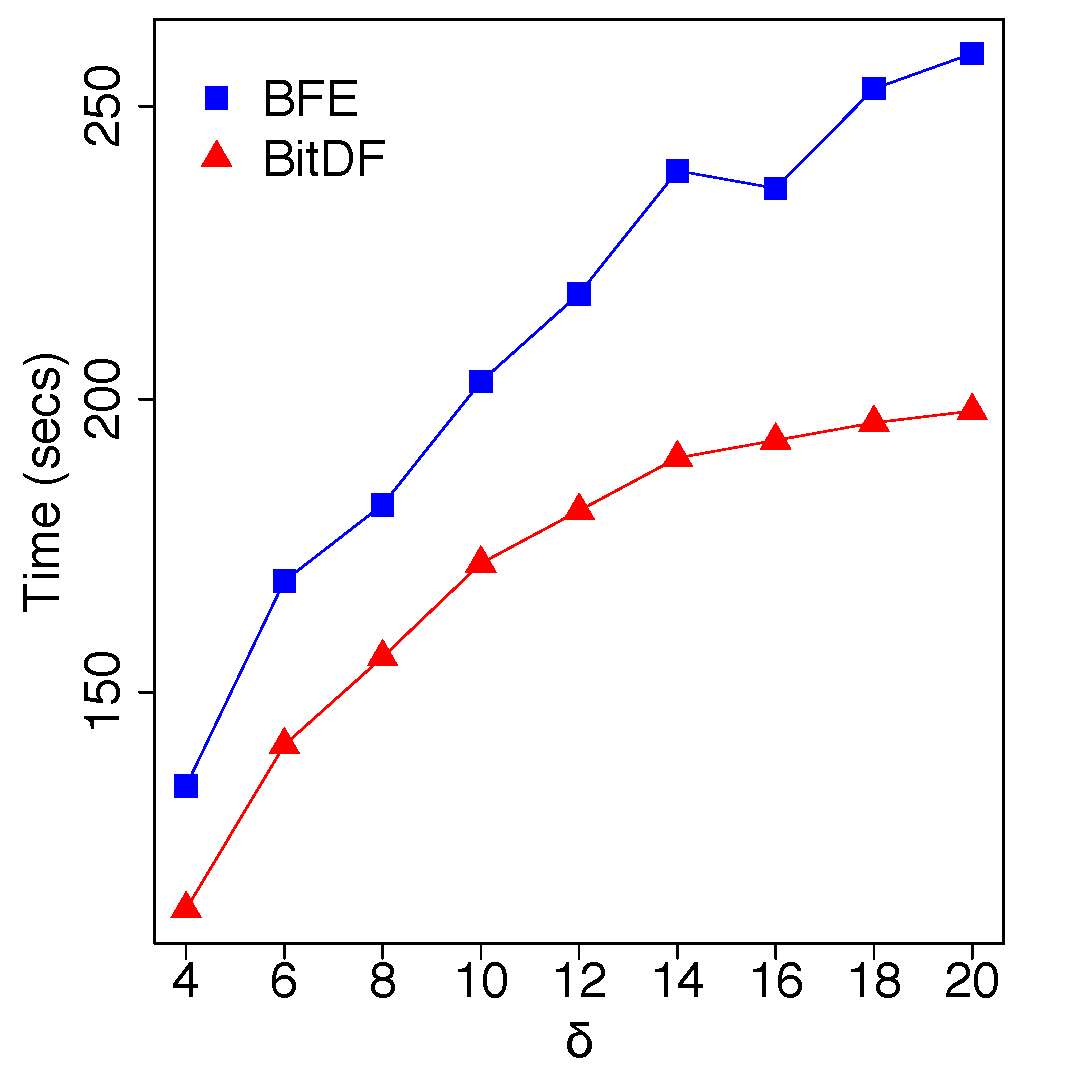
\includegraphics[width=\textwidth]{images/Trucks_n_4_g_1_5_varying_l.eps}
        \caption{$\mu = 4$, $\epsilon = 1.5$ and $\delta$ varying}
        \label{fig:trucks_vary_l}
    \end{subfigure}
    \begin{subfigure}[t]{0.48\textwidth}
        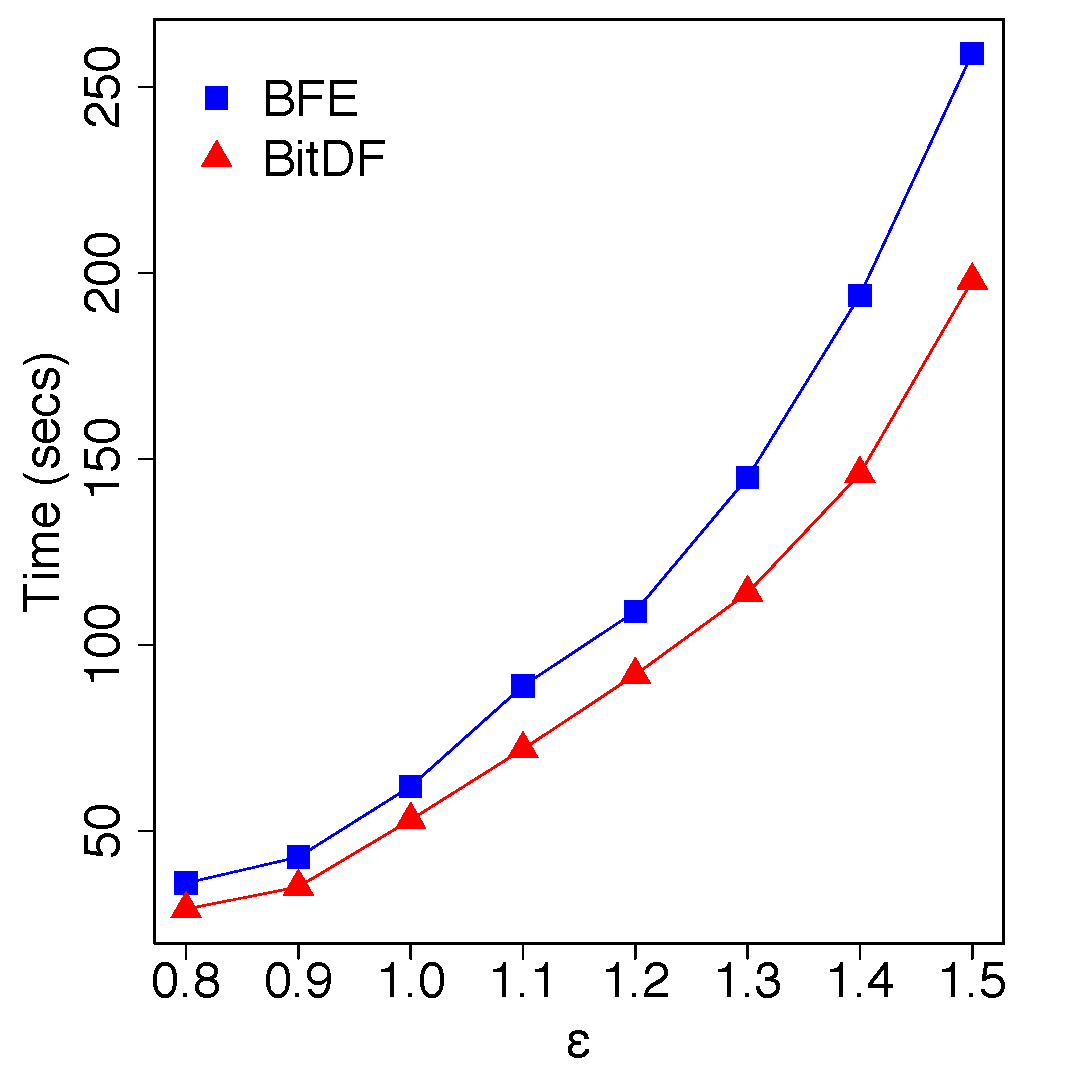
\includegraphics[width=\textwidth]{images/Trucks_n_4_l_20_varying_g.eps}
        \caption{$\mu = 4$, $\delta = 20$ and $\epsilon$ varying}
        \label{fig:trucks_vary_g}
    \end{subfigure}
    \caption{Results varying $\delta$ and $\epsilon$ for Trucks dataset}
    \label{fig:trucks_results}
\end{figure*}

\begin{figure*}[h!]
    \begin{subfigure}[t]{0.48\textwidth}
        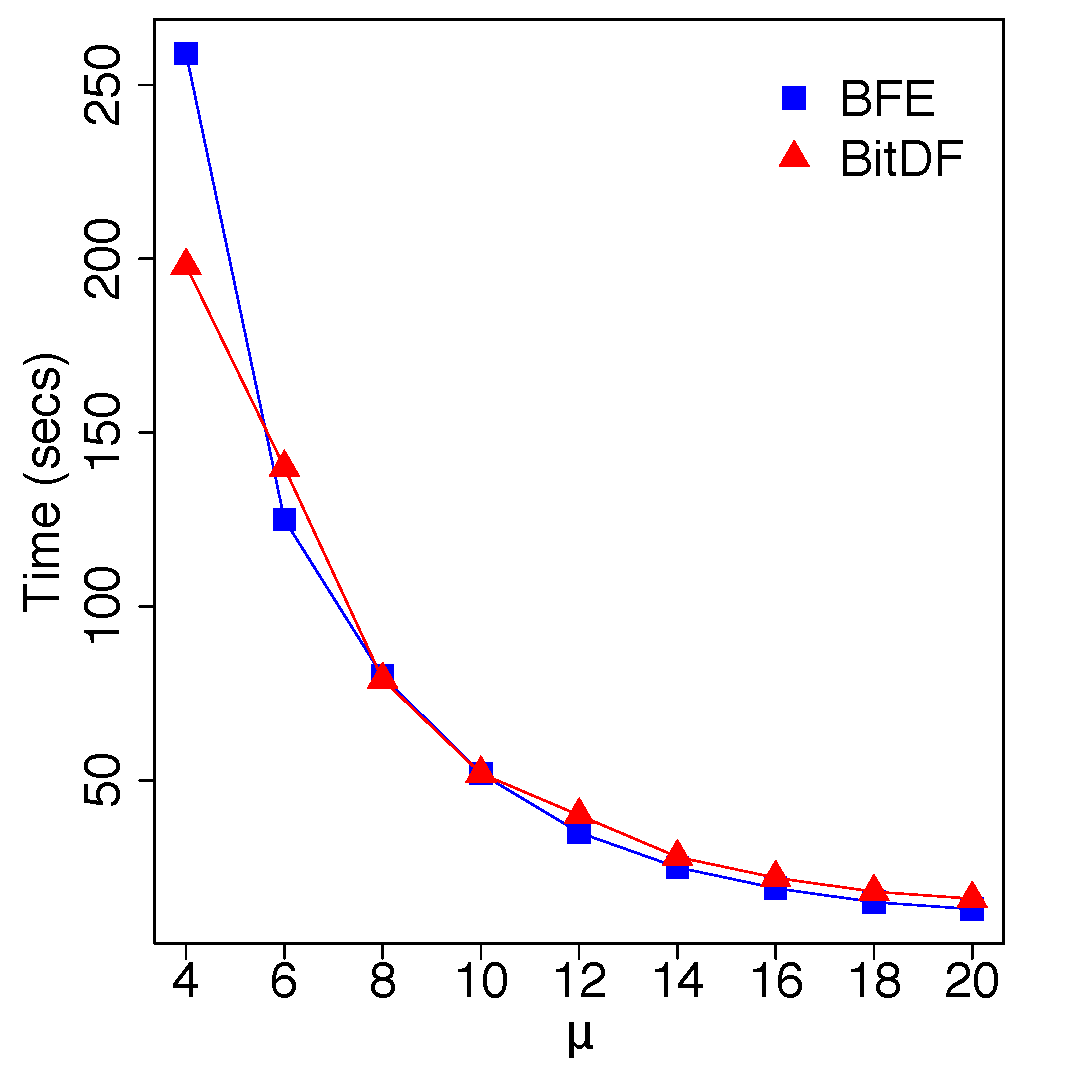
\includegraphics[width=\textwidth]{images/Trucks_l_20_g_1_5_varying_n.eps}
        \caption{$\delta = 20$, $\epsilon = 1.5$ and $\mu$ varying}
        \label{fig:trucks_vary_n}
    \end{subfigure}
    \begin{subfigure}[t]{0.48\textwidth}
        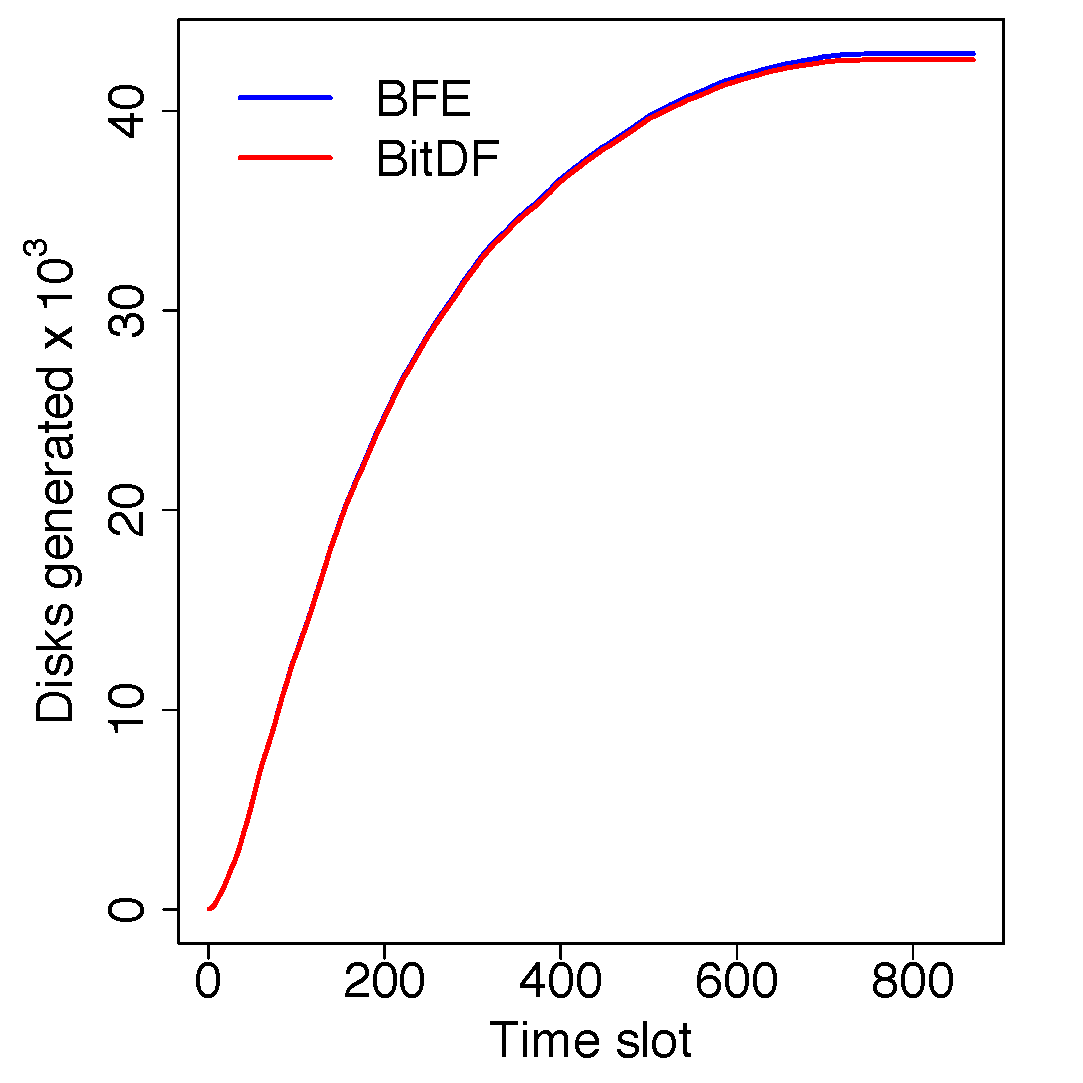
\includegraphics[width=\textwidth]{images/Trucks_d.eps}
        \caption{Cumulative disks by time}
        \label{fig:trucks_disks}
    \end{subfigure}
    \caption{Results varying $\mu$ and number of disks generated over time for Trucks dataset}
    \label{fig:trucks_results2}
\end{figure*}

By looking at \figref{fig:trucks_results} and \figref{fig:trucks_results2}, we can see that we have some gains in
execution time. However, they are not too significant due to the fact that the number of disks generated by each time
slot does not differ too much between BFE and BitDF, as we can see in \figref{fig:trucks_disks}. This happens because
almost all points appear in every single time slot, then buffering and mapping the $O_{id}$ presence in time does not
make a big impact, since we will not be able to filter out disks created with points not being present in $\delta$
consecutive time slots.  \figref{fig:trucks_vary_l} and \figref{fig:trucks_vary_g} show some running time improvements
against BFE, which are backed up by the explanations given at~\ref{sssec:lvariation} and~\ref{sssec:gvariation}. A
different behavior is observed in \figref{fig:trucks_vary_n}, in which BitDF starts better but ends up almost tied with
BFE, which can be explained by~\ref{sssec:nvariation}, but is also very influenced by the dataset modifications.

\section{BerlinMOD Dataset}
\label{sec:berlinmod}
BerlinMOD consists in a traffic generation model \citep{berlinmodpaper} used to create sythentic datasets of moving
objects. This particular dataset that we are analysing was the biggest one that we could find in the set of synthetic
datasets that are available in their website \citep{berlinmod} and consists of 56,127,943 entries and 2000 unique
$O_{id}$.

\begin{figure*}[h!]
    \centering
    \begin{subfigure}[t]{0.48\textwidth}
        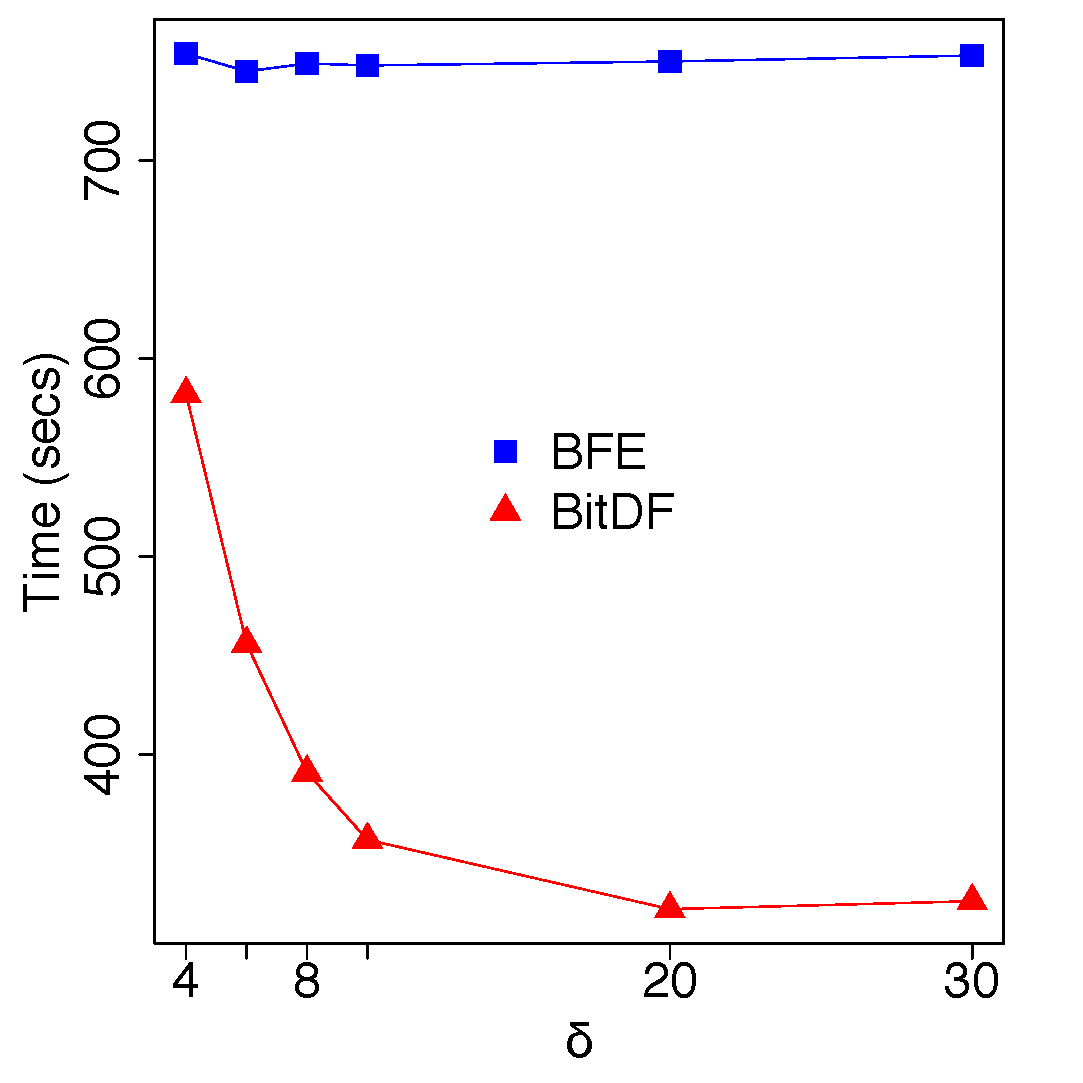
\includegraphics[width=\textwidth]{images/BerlinMOD_n_4_g_100_varying_l.eps}
        \caption{$\mu = 4$, $\epsilon = 100$ and $\delta$ varying}
        \label{fig:berlinmod_vary_l}
    \end{subfigure}
    \begin{subfigure}[t]{0.48\textwidth}
        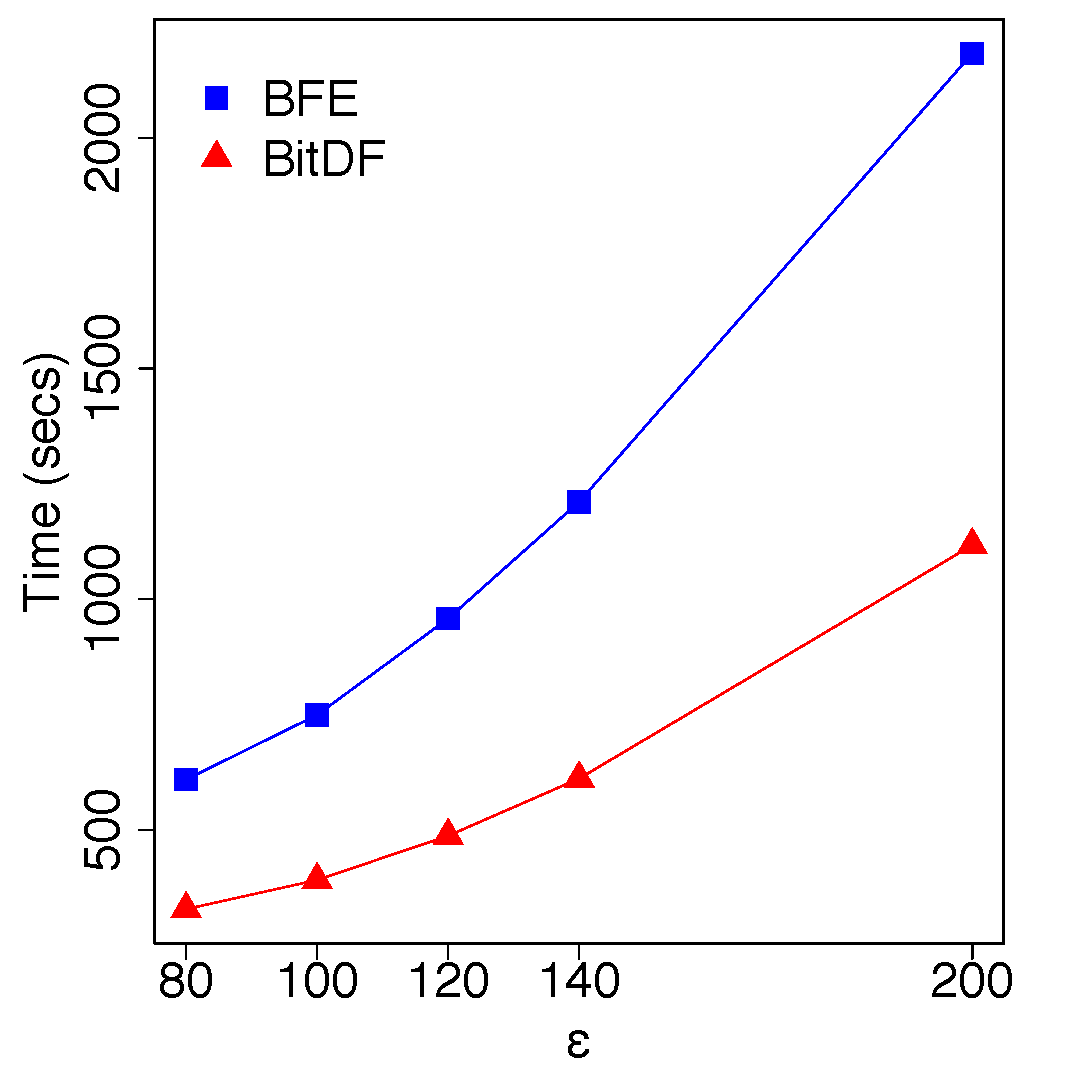
\includegraphics[width=\textwidth]{images/BerlinMOD_n_4_l_8_varying_g.eps}
        \caption{$\mu = 4$, $\delta = 8$ and $\epsilon$ varying}
        \label{fig:berlinmod_vary_g}
    \end{subfigure}
    \caption{Results varying $\delta$ and $\epsilon$ for BerlinMOD dataset}
    \label{fig:berlinmod_results}
\end{figure*}

\begin{figure*}[h!]
    \begin{subfigure}[t]{0.48\textwidth}
        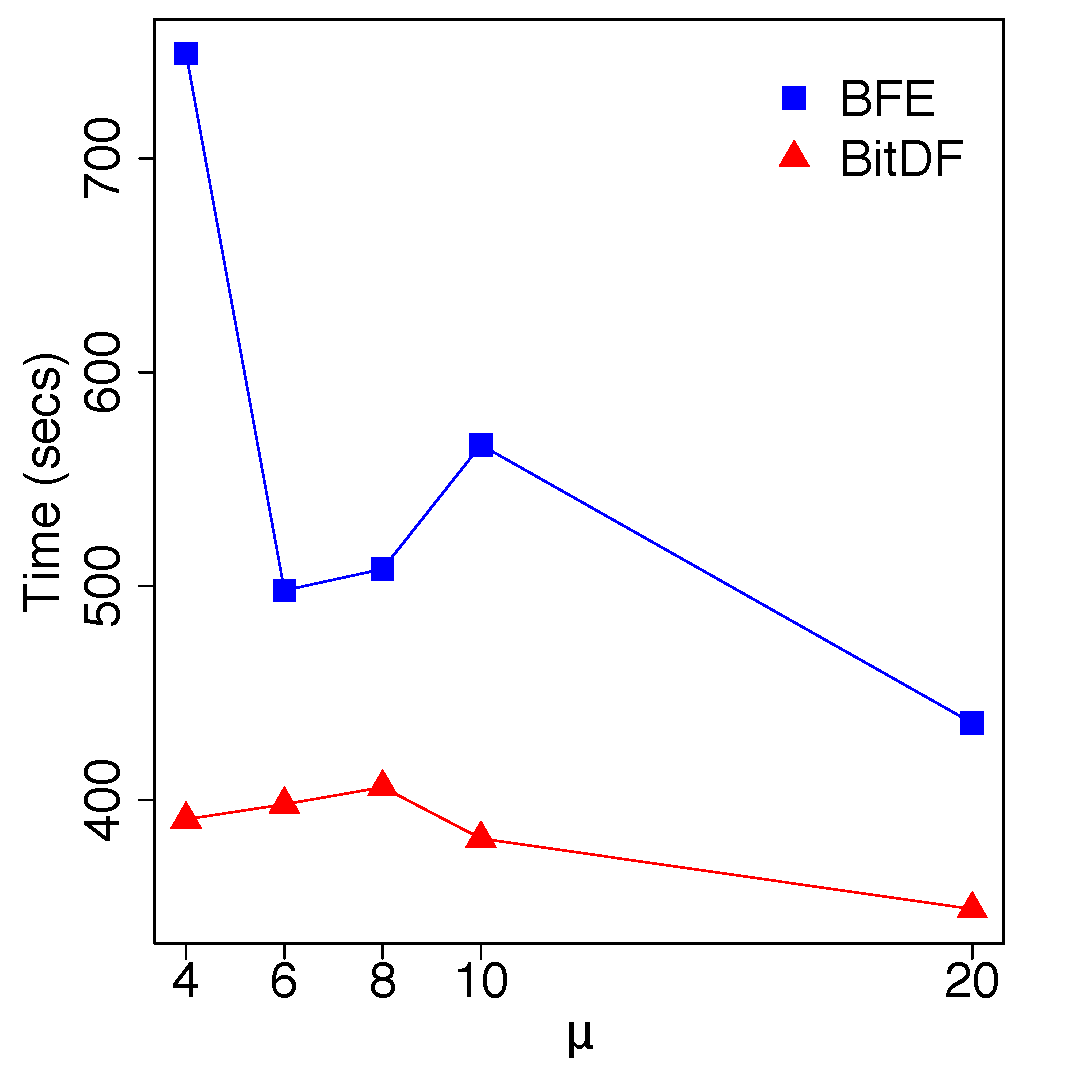
\includegraphics[width=\textwidth]{images/BerlinMOD_l_8_g_100_varying_n.eps}
        \caption{$\delta = 8$, $\epsilon = 100$ and $\mu$ varying}
        \label{fig:berlinmod_vary_n}
    \end{subfigure}
    \begin{subfigure}[t]{0.48\textwidth}
        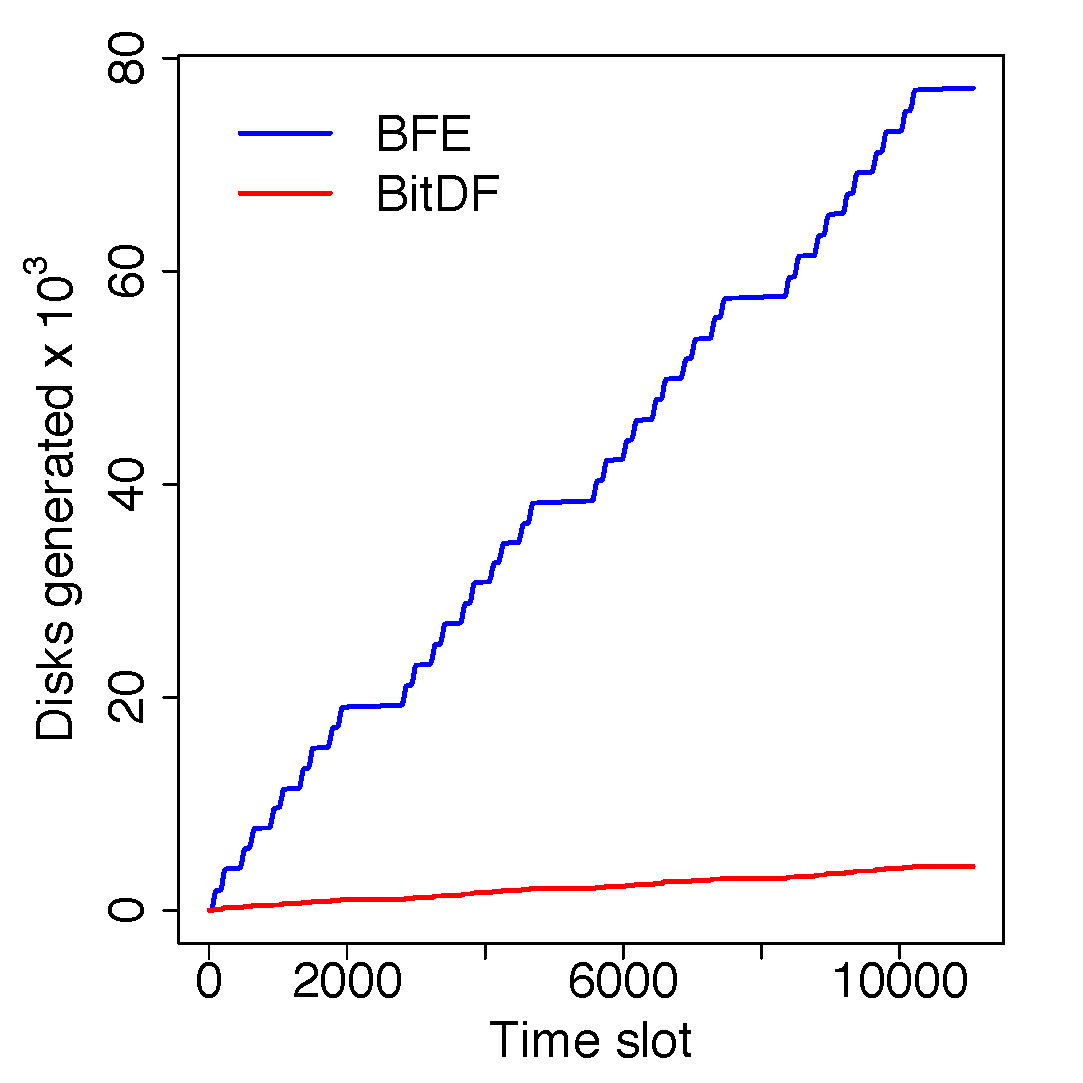
\includegraphics[width=\textwidth]{images/BerlinMOD_d.eps}
        \caption{Cumulative disks by time}
        \label{fig:berlinmod_disks}
    \end{subfigure}
    \caption{Results varying $\mu$ and number of disks generated over time for BerlinMOD dataset}
    \label{fig:berlinmod_results2}
\end{figure*}

As we can see by the results presented in \figref{fig:berlinmod_results} and \figref{fig:berlinmod_results2}, BitDF was
able to achieve great performance gains over BFE, in some cases being 57\% faster (\figref{fig:berlinmod_vary_l}). In
\figref{fig:berlinmod_disks} it is shown that BitDF reduces the cumulative number of disks created over time in 94\%, by
only creating disks that can indeed form flock patterns, which justifies the great improvements that BitDF was able to
get in this dataset. Differently from the results presented in \secref{sec:trucks}, even with a growing $\mu$, BitDF was
able to get great improvements over BFE, ranging from 20\% to 48\%, as depicted in \figref{fig:berlinmod_vary_n}. It is
also worth mentioning the gain in running time that BitDF was able to achieve when we varied the $\epsilon$ parameter,
reaching 48\%, as shown in \figref{fig:berlinmod_vary_g}

\section{TDrive Dataset}
\label{sec:tdrive}
This is a real dataset, having spatio-temporal data describing one week of taxis' trajectories of taxis in Beijing,
China, available in \citep{tdrive}. It has 17,762,489 entries with 10336 unique $O_{id}$.

\begin{figure*}[h!]
    \centering
    \begin{subfigure}[t]{0.48\textwidth}
        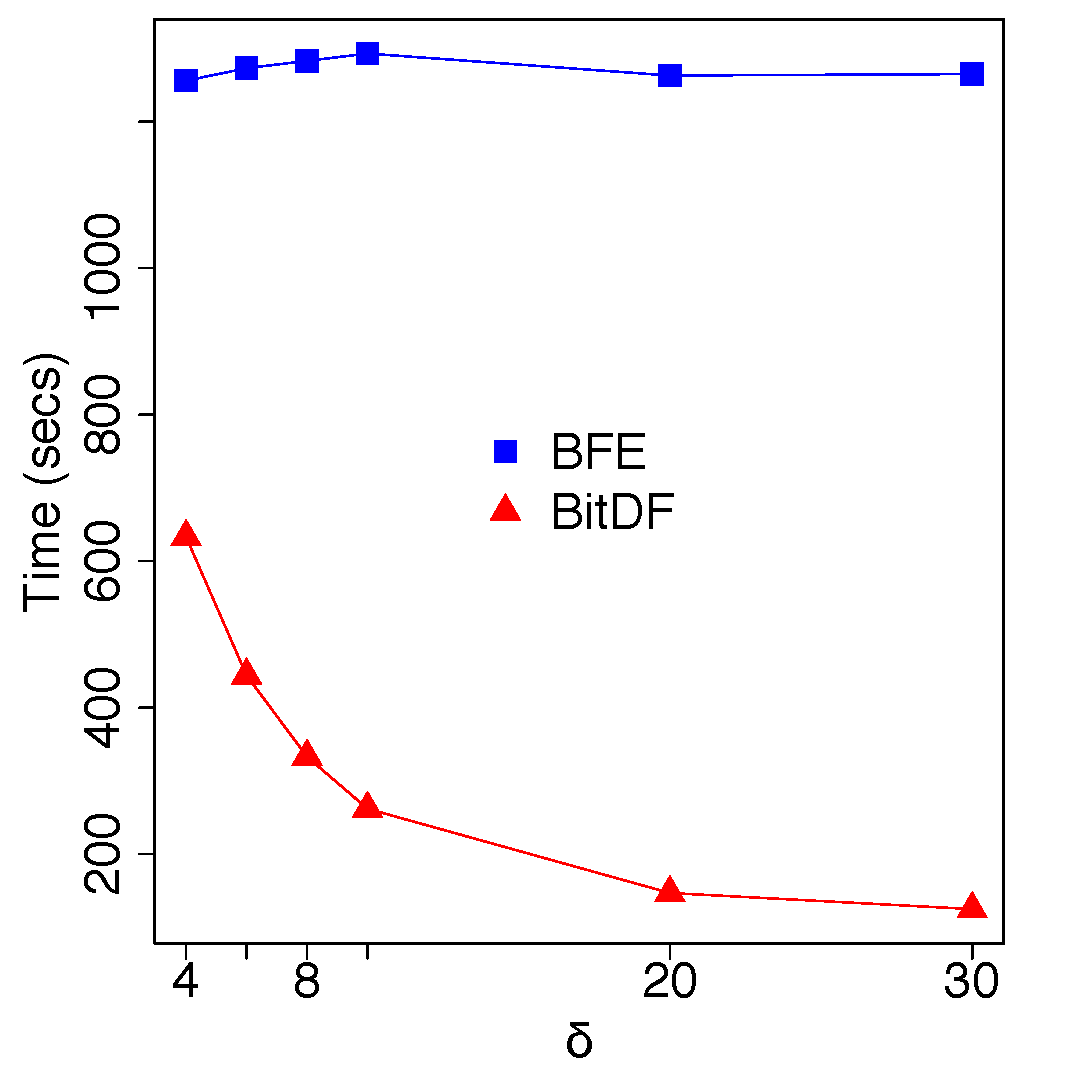
\includegraphics[width=\textwidth]{images/TDrive_n_4_g_100_varying_l.eps}
        \caption{$\mu = 4$, $\epsilon = 100$ and $\delta$ varying}
        \label{fig:tdrive_vary_l}
    \end{subfigure}
    \begin{subfigure}[t]{0.48\textwidth}
        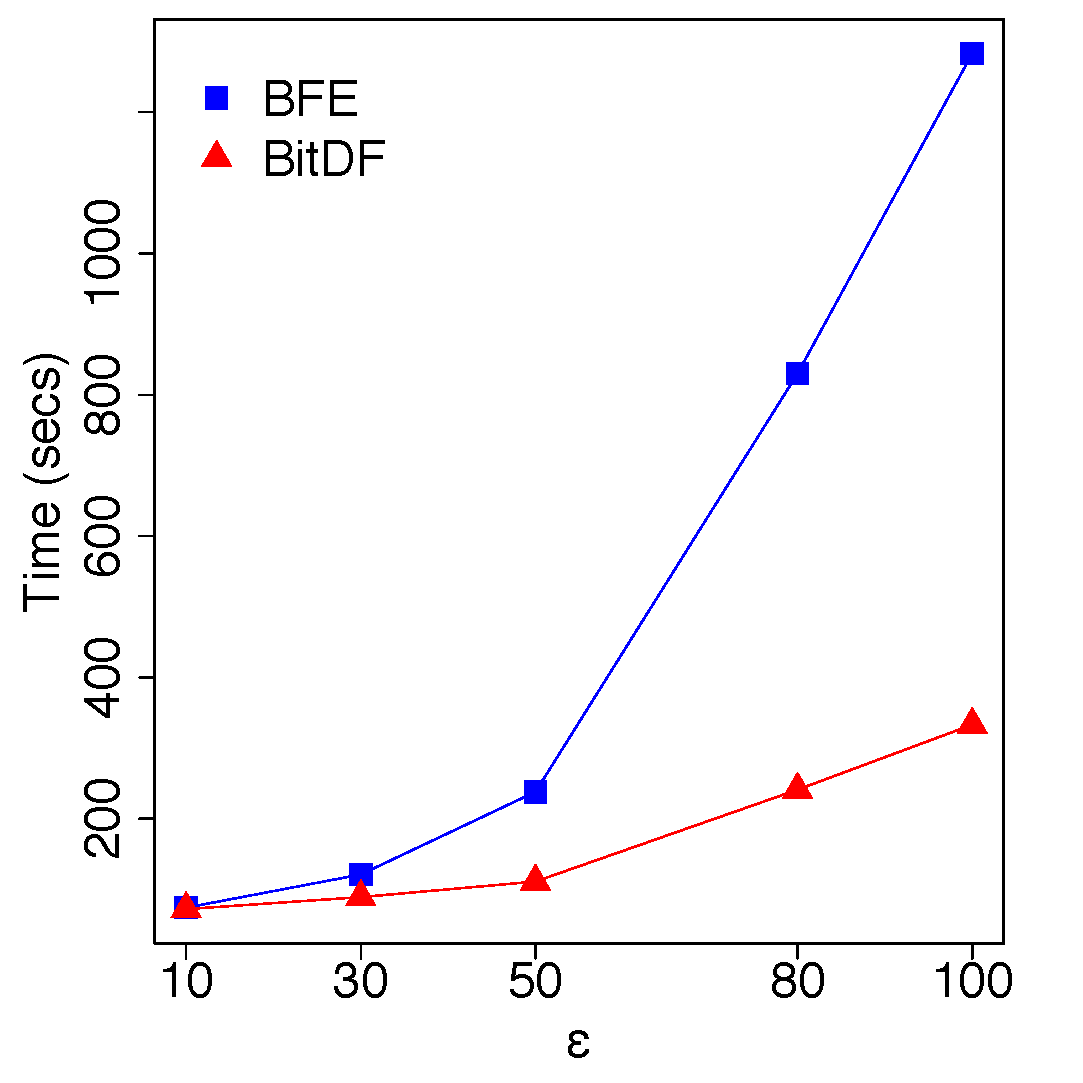
\includegraphics[width=\textwidth]{images/TDrive_n_4_l_8_varying_g.eps}
        \caption{$\mu = 4$, $\delta = 8$ and $\epsilon$ varying}
        \label{fig:tdrive_vary_g}
    \end{subfigure}
    \caption{Results varying $\delta$ and $\epsilon$ for TDrive dataset}
    \label{fig:tdrive_results}
\end{figure*}

One can see by the results presented in \figref{fig:tdrive_results} and \figref{fig:tdrive_results2}, that BitDF was
able to dramatically reduce the execution time, when compared to BFE. When varying the $\delta$ parameter, the running
time improvement was of almost 90\%, droping from 1,2265 seconds to only 125 seconds of processing time, as shown in
\figref{fig:tdrive_vary_l}. Continuing the improvements, in \figref{fig:tdrive_vary_g} we can see that BitDF reduced the
execution time up to 74\% when varying $\epsilon$. Additionally, despite seeing some similar behavior with the other
analyzed datasets (like presented in \secref{sec:trucks}) when varying $\mu$, \figref{fig:tdrive_vary_n} shows that
BitDF was able to improve the execution time by 74\% in some cases. It is also worth noting that the results achieved
are a reflex of the huge decrease of disks that were generated by time, as depicted in \figref{fig:tdrive_disks},
reaching almost 96\% of reduction.

\begin{figure*}[h!]
    \begin{subfigure}[t]{0.48\textwidth}
        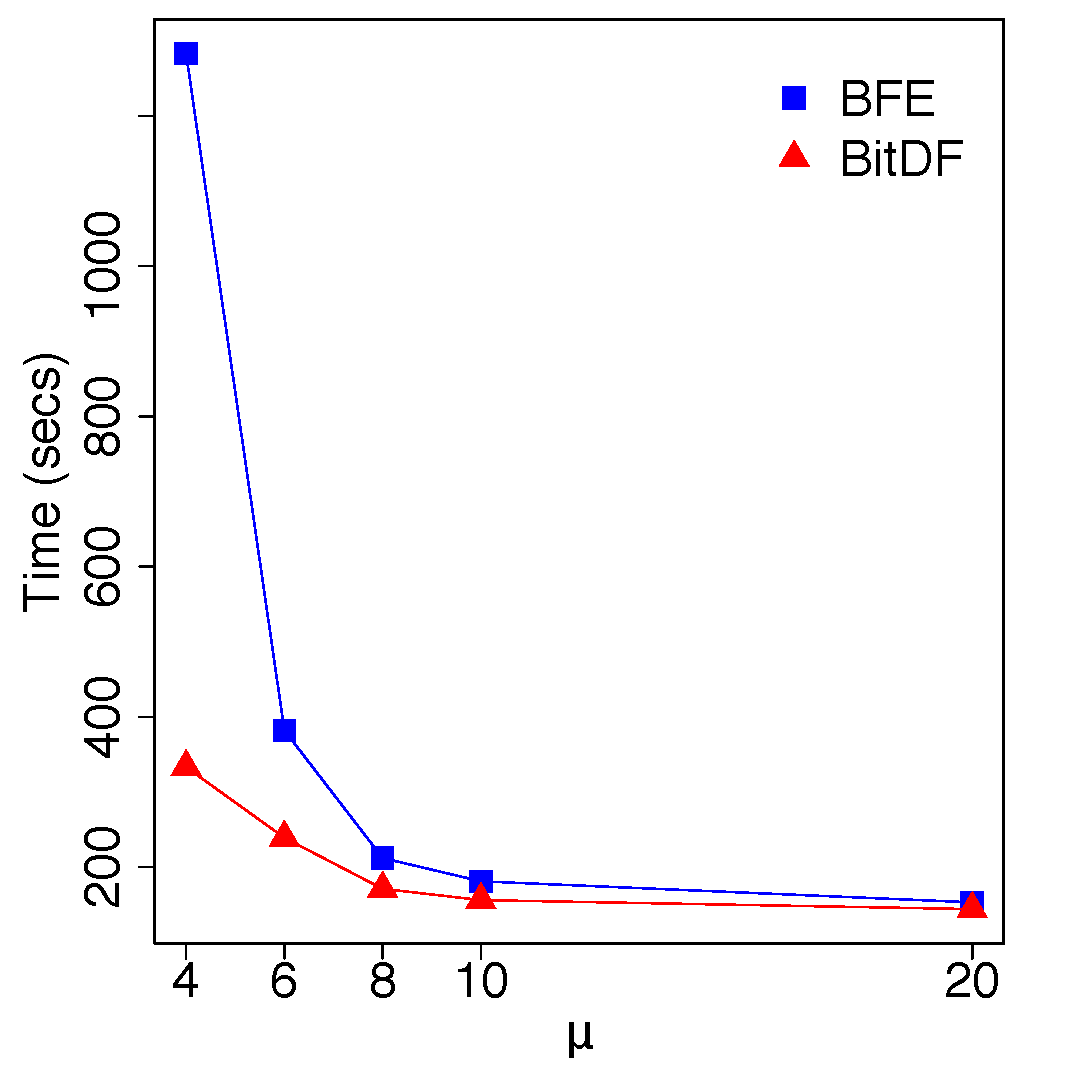
\includegraphics[width=\textwidth]{images/TDrive_l_8_g_100_varying_n.eps}
        \caption{$\delta = 8$, $\epsilon = 100$ and $\mu$ varying}
        \label{fig:tdrive_vary_n}
    \end{subfigure}
    \begin{subfigure}[t]{0.48\textwidth}
        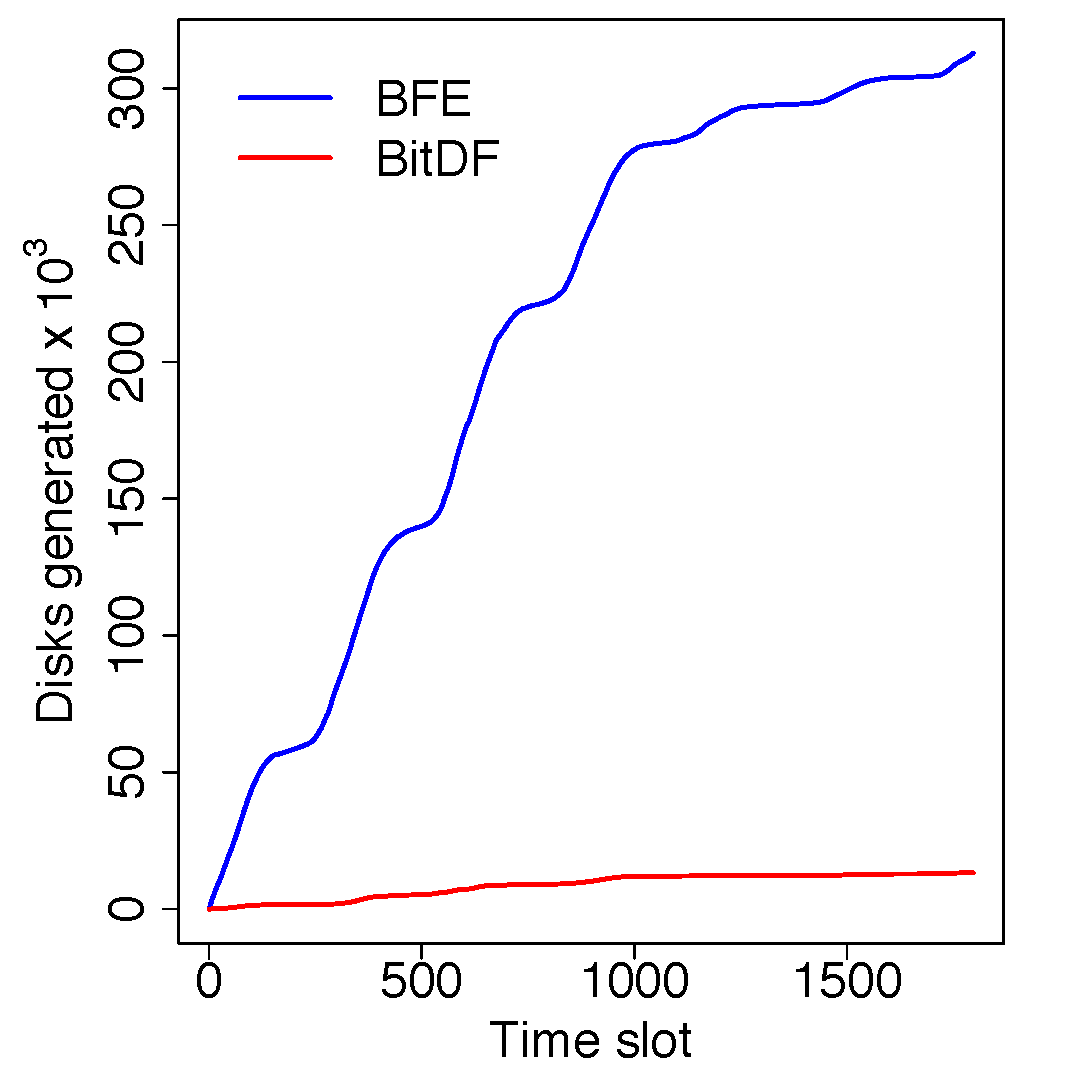
\includegraphics[width=\textwidth]{images/TDrive_d.eps}
        \caption{Cumulative disks by time}
        \label{fig:tdrive_disks}
    \end{subfigure}
    \caption{Results varying $\mu$ and number of disks generated over time for TDrive dataset}
    \label{fig:tdrive_results2}
\end{figure*}

\section{Brinkhoff Dataset}
\label{sec:brinkhoff}
Likewise BerlinMOD, Brinkhoff is also a city traffic generation model \citep{brinkhoffpaper}. We generated a synthetic
dataset using the Minnesota Web-based Traffic Generator \citep{mntg}, having 2000 as the "Starting Vehicles" and 100 as
the "Simulation Time" parameters, which are the largest allowed numbers for them. The result dataset has 314,523 entries
and 7000 unique $O_{id}$.

\begin{figure*}[h!]
    \centering
    \begin{subfigure}[t]{0.48\textwidth}
        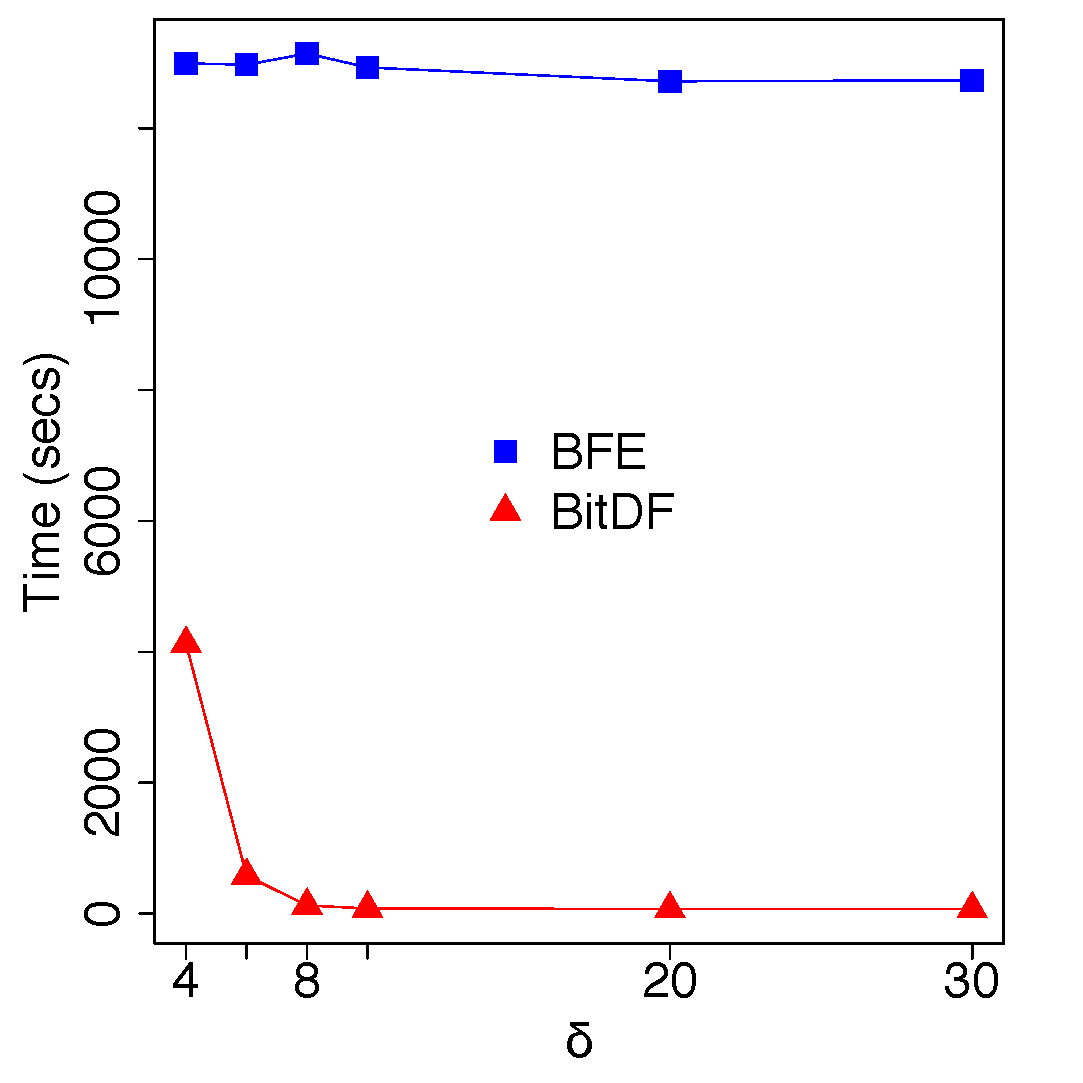
\includegraphics[width=\textwidth]{images/Brinkhoff_n_4_g_200_varying_l.eps}
        \caption{$\mu = 4$, $\epsilon = 200$ and $\delta$ varying}
        \label{fig:brinkhoff_vary_l}
    \end{subfigure}
    \begin{subfigure}[t]{0.48\textwidth}
        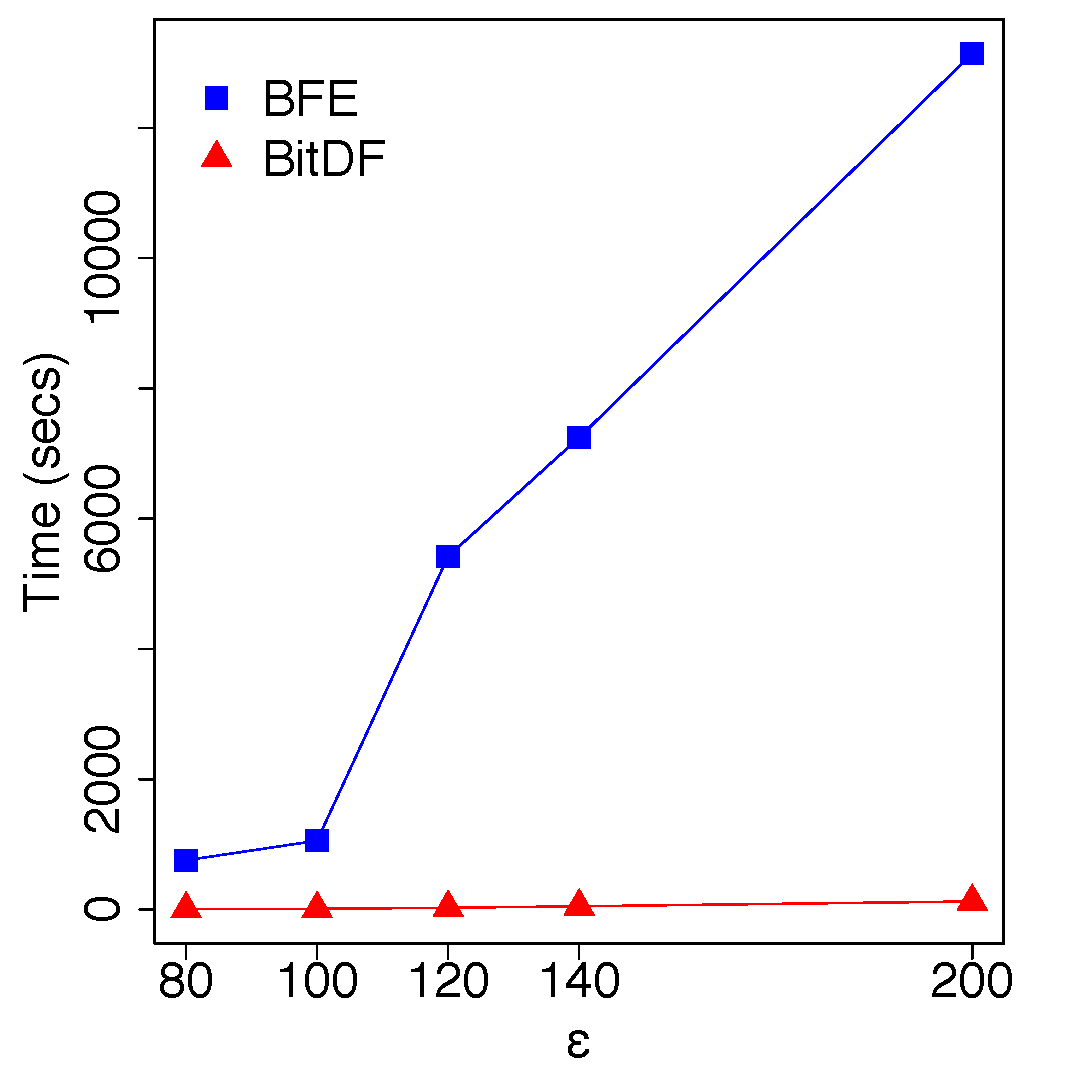
\includegraphics[width=\textwidth]{images/Brinkhoff_n_4_l_8_varying_g.eps}
        \caption{$\mu = 4$, $\delta = 8$ and $\epsilon$ varying}
        \label{fig:brinkhoff_vary_g}
    \end{subfigure}
    \caption{Results varying $\delta$ and $\epsilon$ for Brinkhoff dataset}
    \label{fig:brinkhoff_results}
\end{figure*}

\begin{figure*}[h!]
    \begin{subfigure}[t]{0.48\textwidth}
        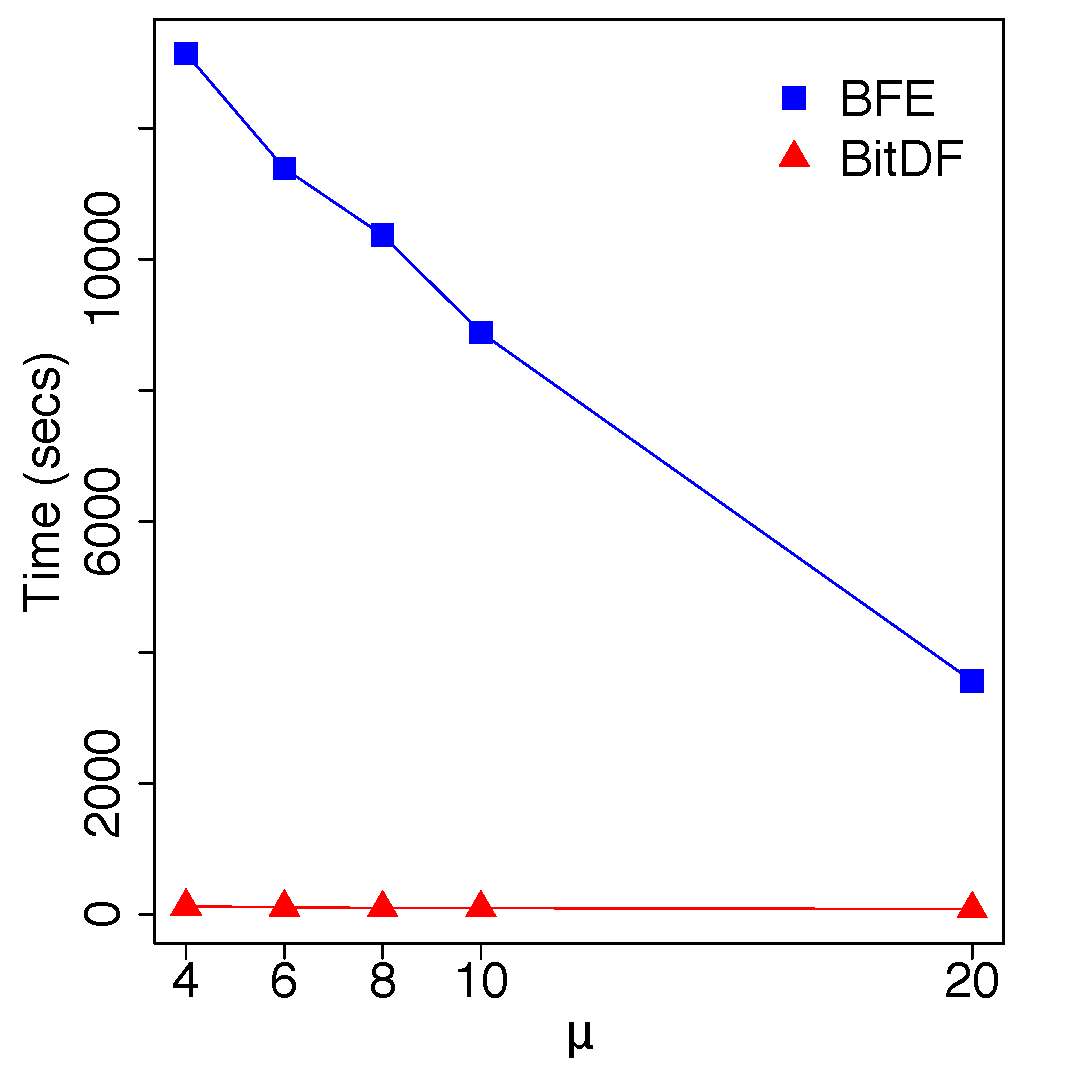
\includegraphics[width=\textwidth]{images/Brinkhoff_l_8_g_200_varying_n.eps}
        \caption{$\delta = 8$, $\epsilon = 200$ and $\mu$ varying}
        \label{fig:brinkhoff_vary_n}
    \end{subfigure}
    \begin{subfigure}[t]{0.48\textwidth}
        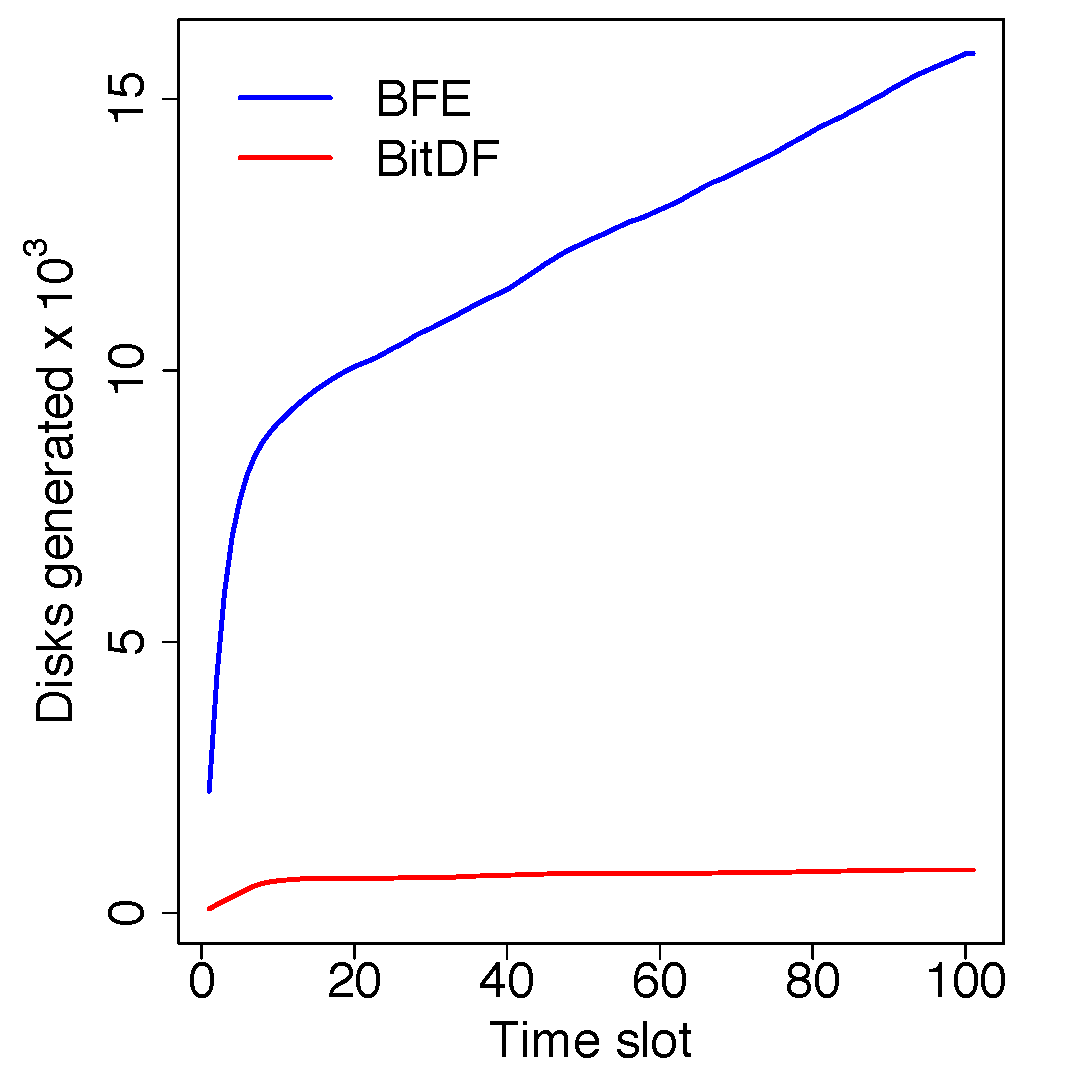
\includegraphics[width=\textwidth]{images/Brinkhoff_d.eps}
        \caption{Cumulative disks by time}
        \label{fig:brinkhoff_disks}
    \end{subfigure}
    \caption{Results varying $\mu$ and number of disks generated over time for Brinkhoff dataset}
    \label{fig:brinkhoff_results2}
\end{figure*}

The results achieved with this dataset were the best that BitDF was able to get amongst the other datasets analyzed in
this thesis, as one can notice by looking to \figref{fig:brinkhoff_results} and \figref{fig:brinkhoff_results2}. There
were huge drops in execution time, as depicted in \figref{fig:brinkhoff_vary_l}, where BitDF analyzed the whole dataset
in only 69 seconds, while BFE took 12,732 seconds, representing an improvement of 99.5\%. Another great running time
improvement of 99\% can be seen when we varied the $\epsilon$ parameter, as shown in \figref{fig:brinkhoff_vary_g},
droping from 13,141 seconds to 125 seconds. We can see in \figref{fig:brinkhoff_vary_n} that even with the variation of
$\mu$, BitDF was able to show huge improvement, with results ranging from 98\% to 99\% of CPU time reduction.
Additionally, we can see in \figref{fig:brinkhoff_disks} that we were able to reduce the number of disks by 95\%, what
is a huge improvement and is reflecting directly in the running time improvements that we could see with this dataset.

% Multi-thread evaluations
\section{Multi-threaded evaluation}
After implementing the architecture proposed in \secref{sec:architecture}, evaluating it in \chapref{chp:results} and
seeing great improvements in the running time when compared with other algorithms, we decided to test how our system
would perform by taking advantage of the multi-core paradigm that is been widely used nowadays. We then took a step
further and implement a new Data Processor, that we called Parallel Flock Processor (PFP). PFP was implemented having in
mind the multi-threaded model described in \secref{subsec:multithread}, which we call BitDF Multi-treaded (BitDF MT).

In order to see how BitDF MT would perform, we took the worst performances of BitDF for each dataset, from
\chapref{chp:results}, and compared it with BitDF MT running with different number of worker threads executing in
parallel. It is important to notice that when we say that we are running with 4 worker threads, we are actually running
with 8 threads: 4 $c_t$ threads processing different EGCs plus one $d_t$ thread (attached to its $c_t$ thread)
processing the disks generated by its parent $c_i$.

Our benchmarks were executed in a different machine from that one mentioned in the beginning of \chapref{chp:results},
in a way that we opted to get a better multi-core processor setup. With that in mind, we ran our experiments in a Linux
box, running Ubuntu 16.04 LTS, having an Intel Xeon CPU, with 2.3 GHz and 4 physical cores, using Intel Hyper-Threading
technology \citep{hyper} meaning that we would theoretically have 8 different processing units.

Below we will present the benchmarks that were run for each dataset already seen in \chapref{chp:results}, namely
Trucks, TDrive, BerlinMOD and Brinkhoff. For each of the aforementioned datasets, we ran BitDF MT with the same
parameters as the longest BitDF run presented in \chapref{chp:results}, varying the threads from 1 (pure BitDF) to 30.
With variations of 1 worker thread from 1 to 10, 2 worker threads from 10 to 20 and 5 worker threads from 20 to 30. We
set the result of BitDF (1 thread) as being 100\% of the total executing time and highlighted with red color and all
BitDF MT runs are in blue, always being a percentage of the highlighted result. It is worth mentioning that here we are
only evaluating the running time of BitDF MT, because the number of generated disks will be the same as we have seen in
the previous results shown for BitDF in \chapref{chp:results}, since we are still using BitDF as the base flock
processor. Additionally, in order to have a better idea on how BitDF MT outperforms BitDF and BFE, we show some graphs
depicting the running time of them together, for each dataset. For our BitDF MT, we picked 5 and 7 as the number of
worker threads, since those are the values that show the best peformance overall.

First we present the results for the Trucks dataset, which we ran with the following parameters (based on previous
results from \secref{sec:trucks}): $\mu=4$, $\delta=20$ and $\epsilon=1.5$. That dataset would be the most difficult one
to show running time improvements due to its small size and running times being already fast (with the longest one being
around 200 seconds for BitDF). Despite that, we can see in \figref{fig:trucks_threads} that we were able to reduce as
much as 51\% when running with 5 $c_t$ threads, which totalize 10 threads. After that we can see that we could stay
almost stable, not gaining any performance but also not deteriorating it too much. Having it becoming stable is an
expected result, as the processor would start to schedule and pause threads execution, because of having all its
resources busy, as the number of executing threads exceeds too much the number of available processing units.

\begin{figure*}[h!]
    \centering
    \begin{subfigure}[t]{0.49\textwidth}
        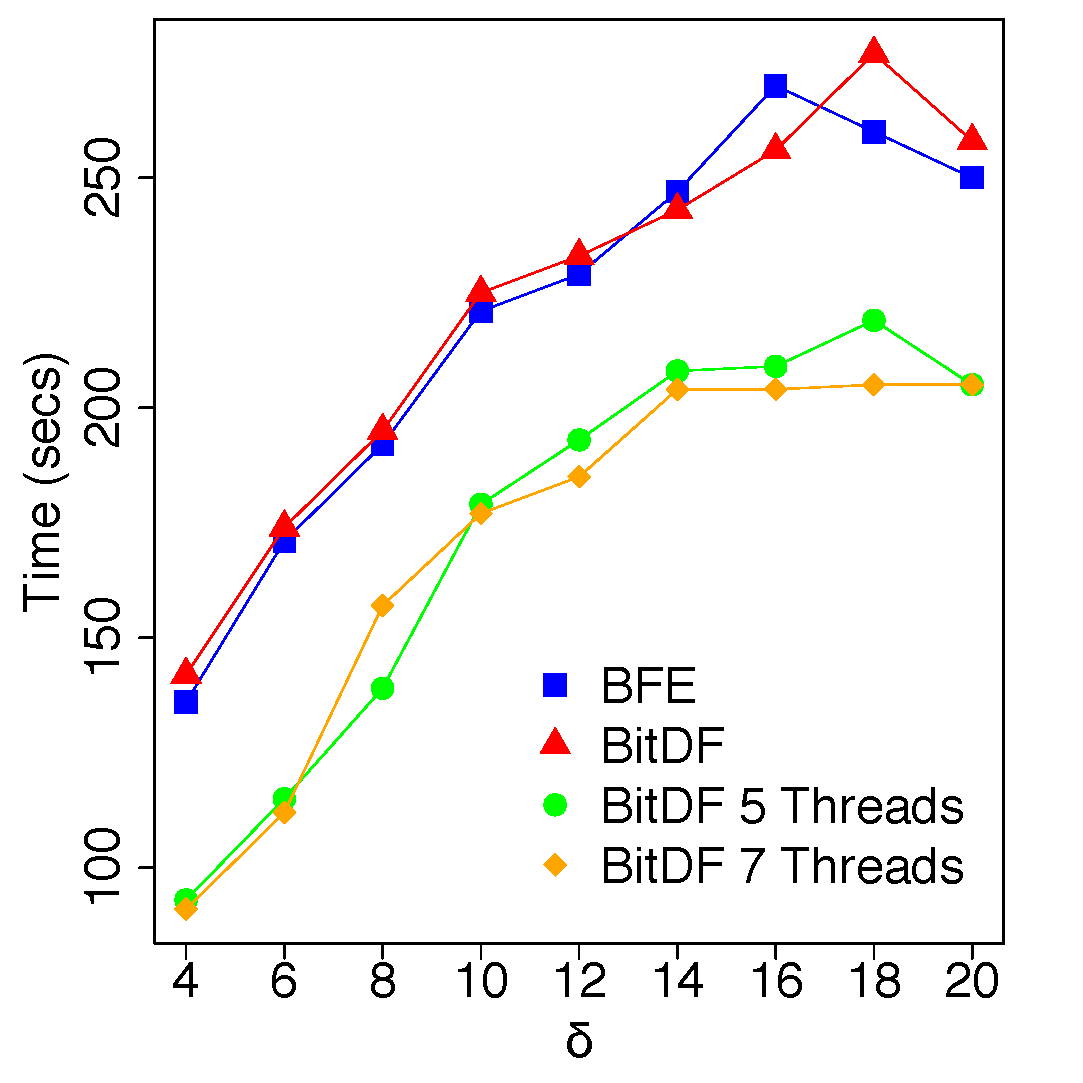
\includegraphics[width=\textwidth]{images/Trucks_complete_varying_l.eps}
        \caption{$\mu = 4$, $\epsilon = 1.5$ and $\delta$ varying}
        \label{fig:trucks_complete_vary_l}
    \end{subfigure}
    \begin{subfigure}[t]{0.49\textwidth}
        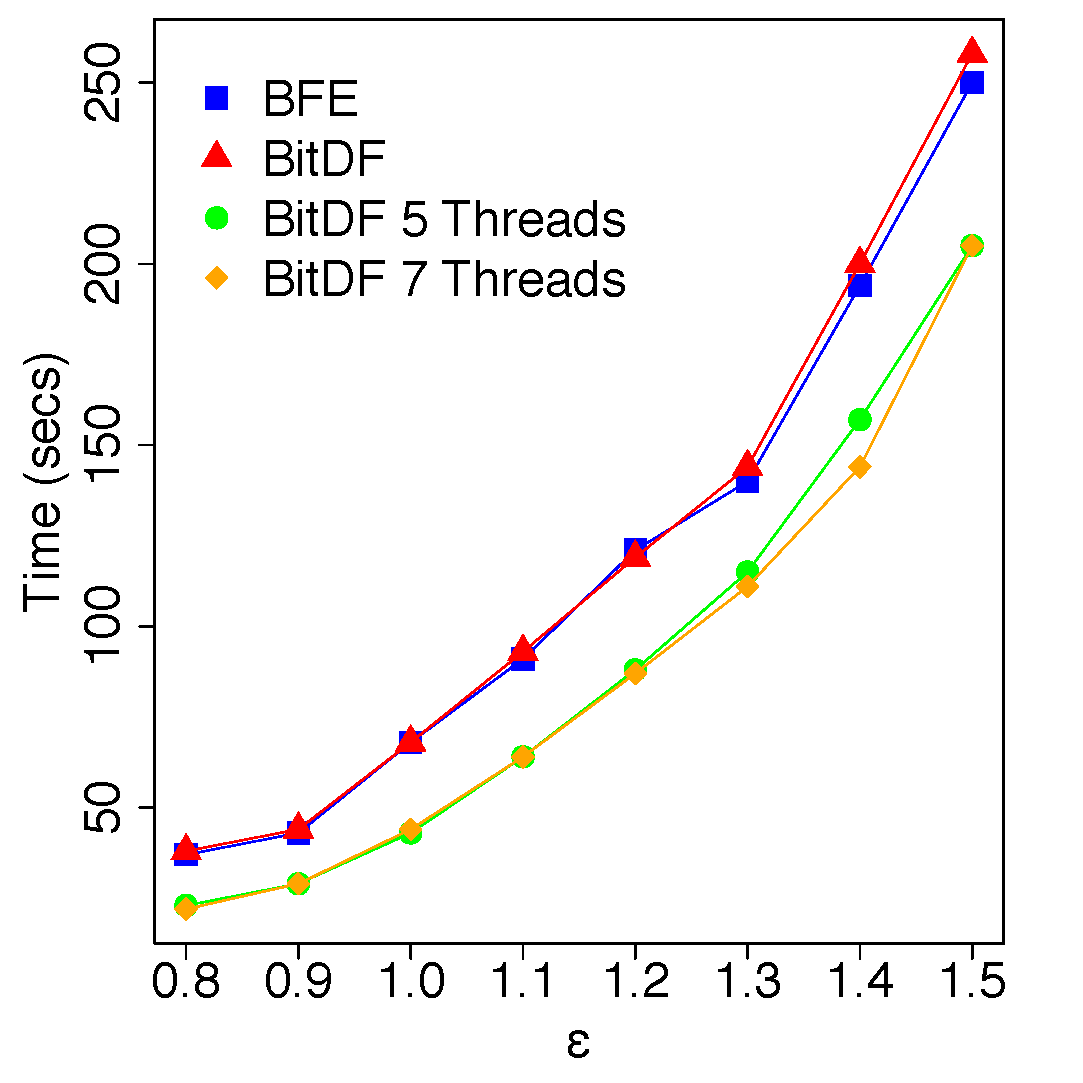
\includegraphics[width=\textwidth]{images/Trucks_complete_varying_g.eps}
        \caption{$\mu = 4$, $\delta = 20$ and $\epsilon$ varying}
        \label{fig:trucks_complete_vary_g}
    \end{subfigure}
    \caption{Results varying $\delta$ and $\epsilon$ for Trucks dataset}
    \label{fig:trucks_complete_results}
\end{figure*}

\figref{fig:trucks_complete_results} and \figref{fig:trucks_complete_vary_n} show that we were able to achieve more
meaningful results with BitDF MT, than those presented in \secref{sec:trucks} and that the improvements obtained with
BitDF MT runing with both 5 and 7 worker threads were almost the same. We could reduce the running time of BitDF by 18\%
when varying $\mu$ (\figref{fig:trucks_complete_vary_n}) and $\epsilon$ (\figref{fig:trucks_complete_vary_g}) and by
30\% when varying $\delta$ (\figref{fig:trucks_complete_vary_l}).

\begin{figure}[h!]
    \centering
    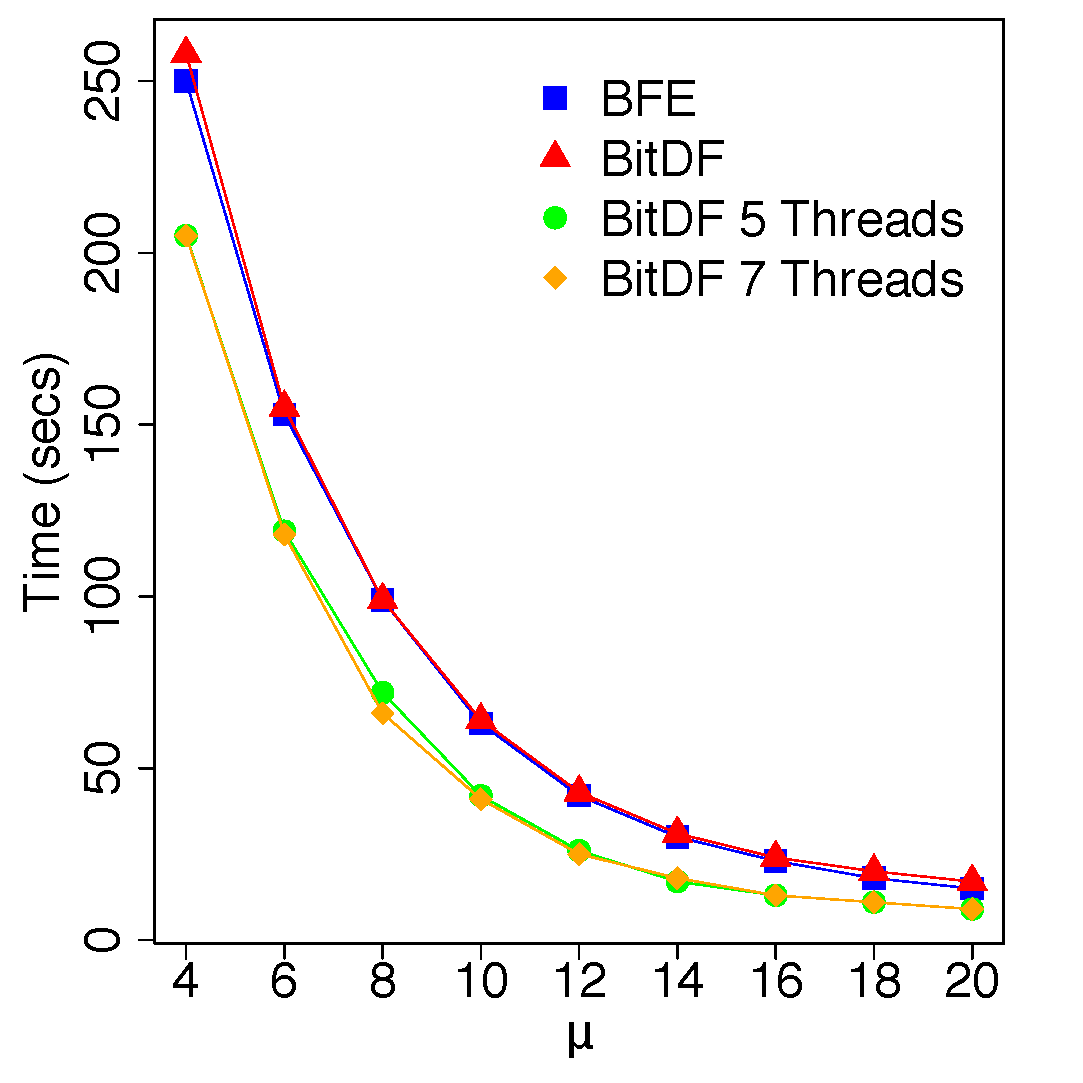
\includegraphics[width=0.5\textwidth]{images/Trucks_complete_varying_n.eps}
    \caption{Results having $\delta = 20$, $\epsilon = 1.5$ and $\mu$ varying for the Trucks dataset}
    \label{fig:trucks_complete_vary_n}
\end{figure}

\begin{figure}[h!]
    \centering
    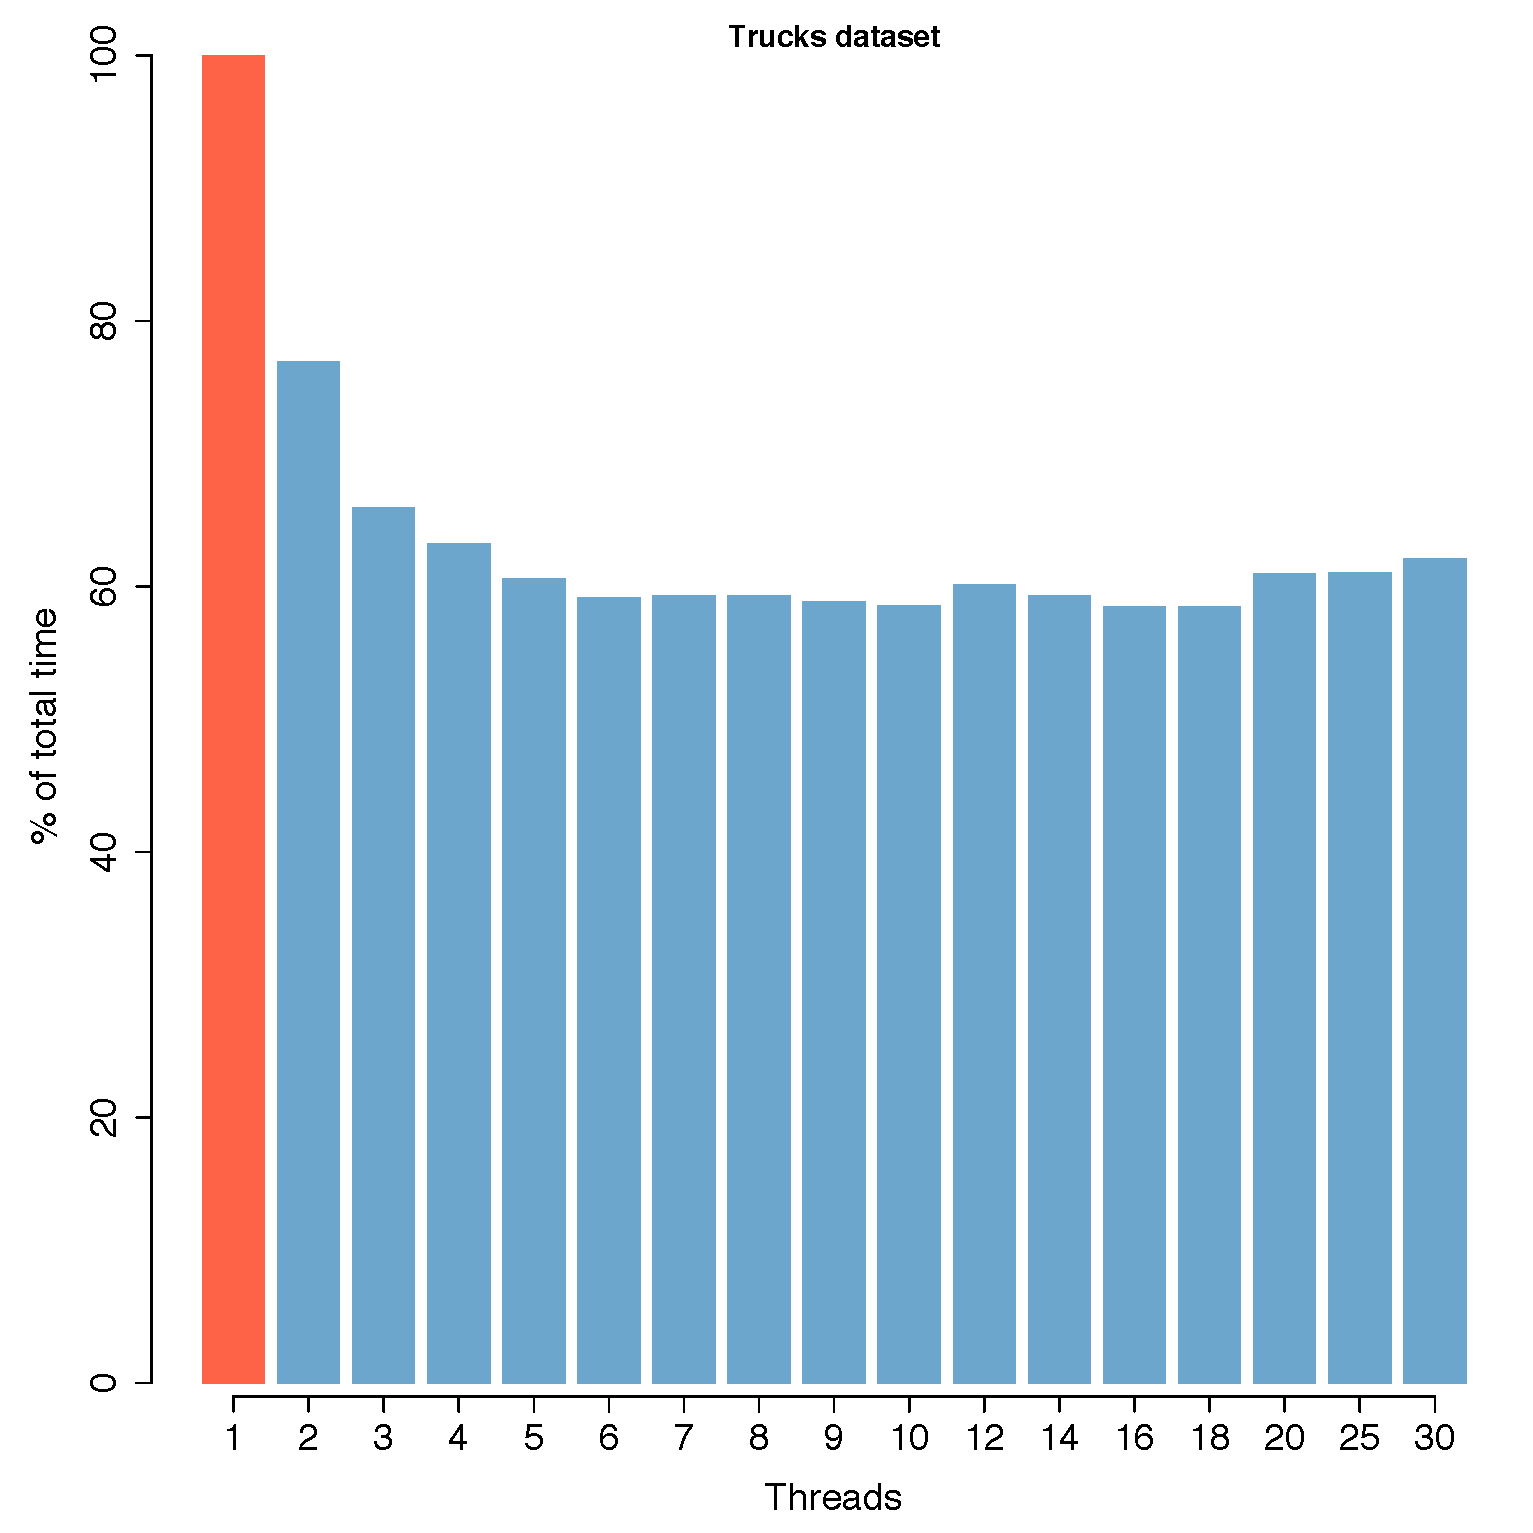
\includegraphics[width=0.7\textwidth]{images/Trucks_thread.eps}
    \caption{Execution time reduction by number of threads for the Trucks dataset}
    \label{fig:trucks_threads}
\end{figure}

In \figref{fig:berlinmod_threads}, we show the graph with the results for the BerlinMOD dataset. Due to its large size
and somewhat long execution times (as previously presented in \secref{sec:berlinmod}) we expected to obtain good results
in running BitDF in a multi-threaded fashion. We have set our parameters to have the following values: $\mu=4$,
$\delta=8$ and $\epsilon=200$, as we had those resulting in the longest running time (around 1000 seconds). It is
noticed by \figref{fig:berlinmod_threads} that the results also tend to stabilize when we reach 5 worker threads (10 in
total), but we reach our best running time with 8 worker threads, with an improvement of 62\%. It is also seen that the
running time starts to getting worse as we exceed the number of processing units too much (shown when BitDF is executing
with 30 worker threads, being 60 in total).

\begin{figure*}[h!]
    \centering
    \begin{subfigure}[t]{0.49\textwidth}
        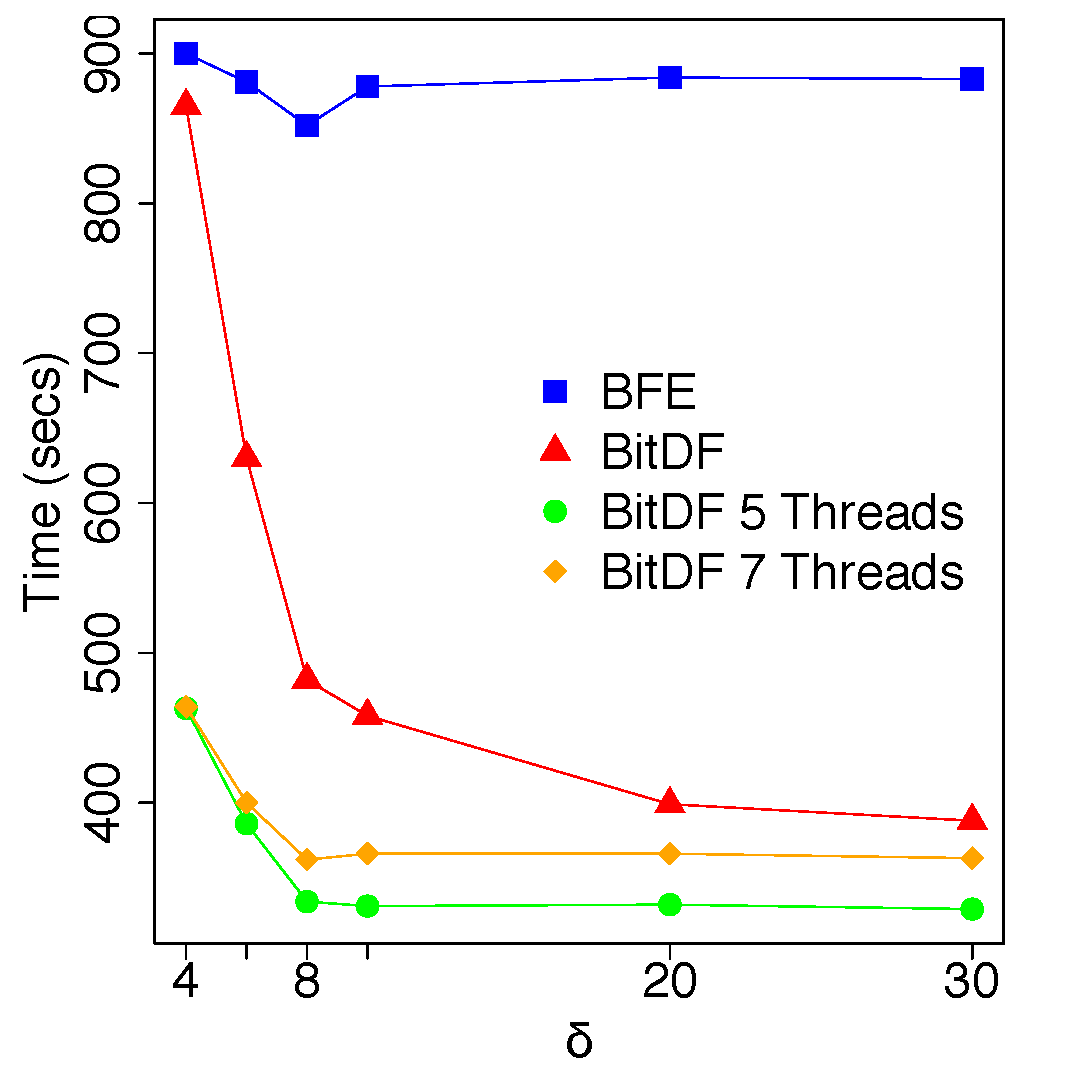
\includegraphics[width=\textwidth]{images/BerlinMOD_complete_varying_l.eps}
        \caption{$\mu = 4$, $\epsilon = 100$ and $\delta$ varying}
        \label{fig:berlinmod_complete_vary_l}
    \end{subfigure}
    \begin{subfigure}[t]{0.49\textwidth}
        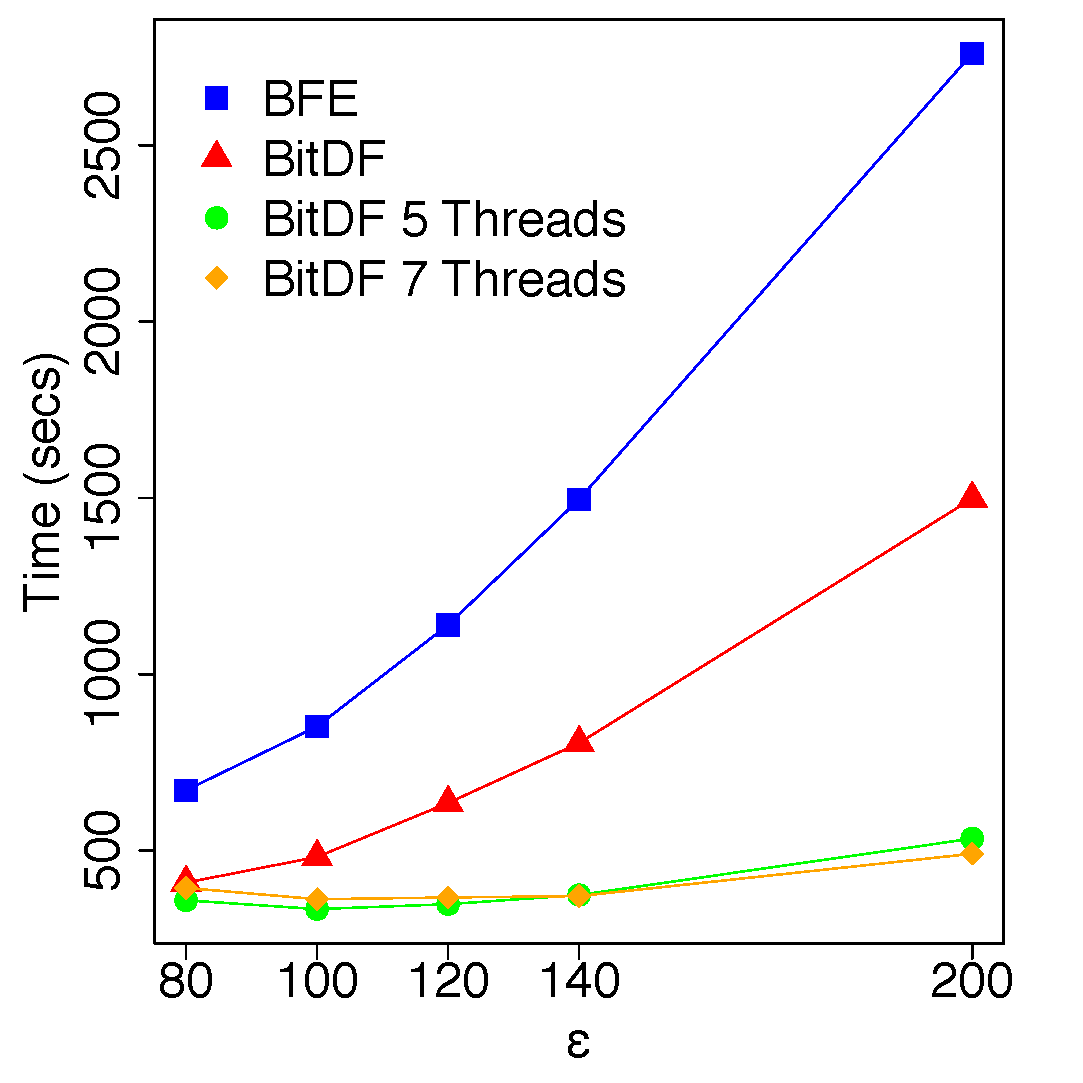
\includegraphics[width=\textwidth]{images/BerlinMOD_complete_varying_g.eps}
        \caption{$\mu = 4$, $\delta = 8$ and $\epsilon$ varying}
        \label{fig:berlinmod_complete_vary_g}
    \end{subfigure}
    \caption{Results varying $\delta$ and $\epsilon$ for BerlinMOD dataset}
    \label{fig:berlinmod_complete_results}
\end{figure*}

\begin{figure}[h!]
    \centering
    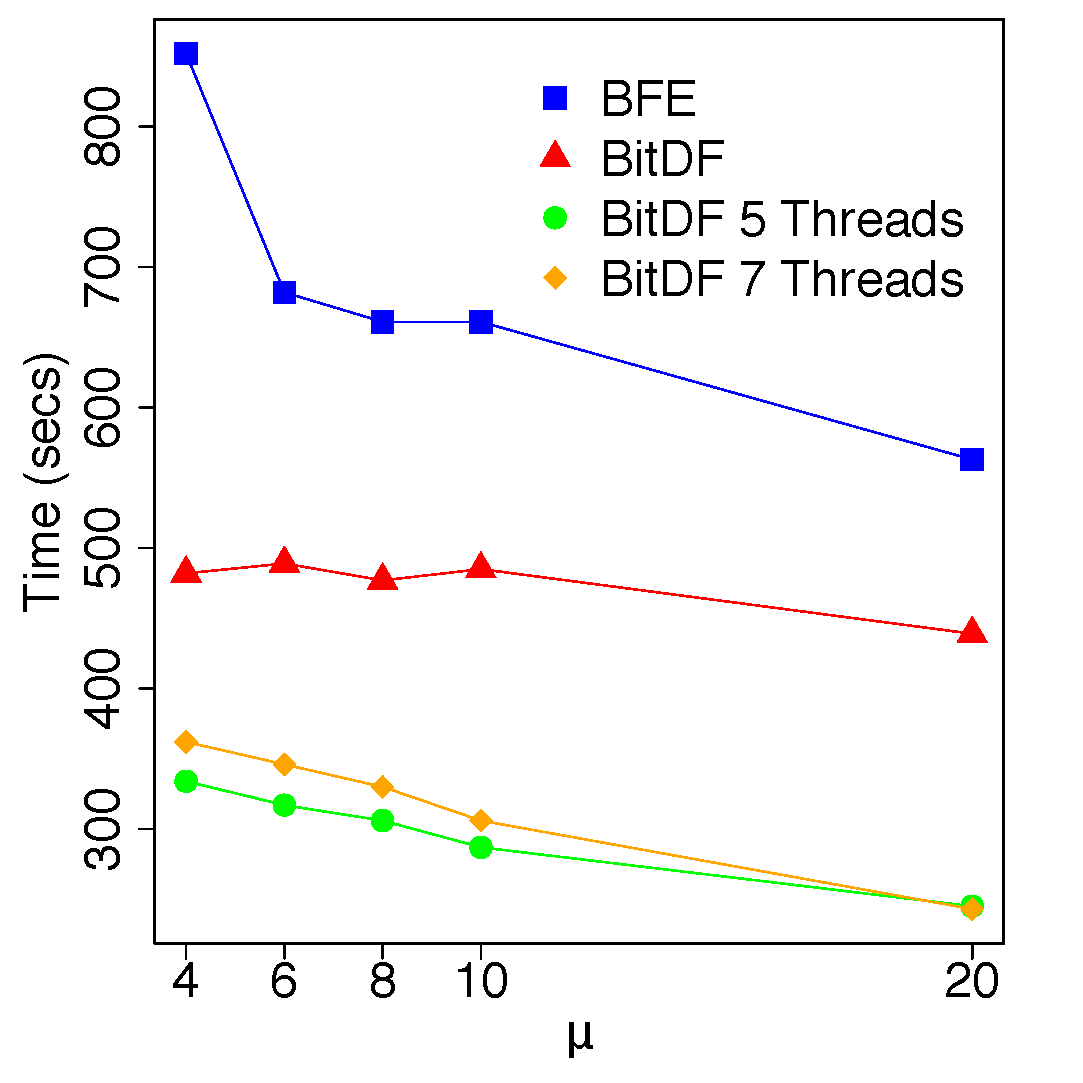
\includegraphics[width=0.5\textwidth]{images/BerlinMOD_complete_varying_n.eps}
    \caption{Results having $\delta = 8$, $\epsilon = 100$ and $\mu$ varying for the BerlinMOD dataset}
    \label{fig:berlinmod_complete_vary_n}
\end{figure}

By looking at \figref{fig:berlinmod_complete_results} and \figref{fig:berlinmod_complete_vary_n}, one can see that
where BitDF had the worst results is where BitDF MT was able to show how a good multi-threaded remodeling is important
in order to get the most out of multi-core architecture. BitDF MT improved the running time of BitDF by 50\% when
running with both 5 and 7 worker threads, as shown in \figref{fig:berlinmod_complete_vary_l}. BitDF MT also achieved
good results when we varied the $\mu$ parameter, having 45\% of running time decrease as it is depicted in
\figref{fig:berlinmod_complete_vary_n}. Last, but definitely not least, we can se in
\figref{fig:berlinmod_complete_vary_l} that BitDF MT improved the running time of BitDF by 70\%, with both 5 and 7
worker threads.

\begin{figure}[h!]
    \centering
    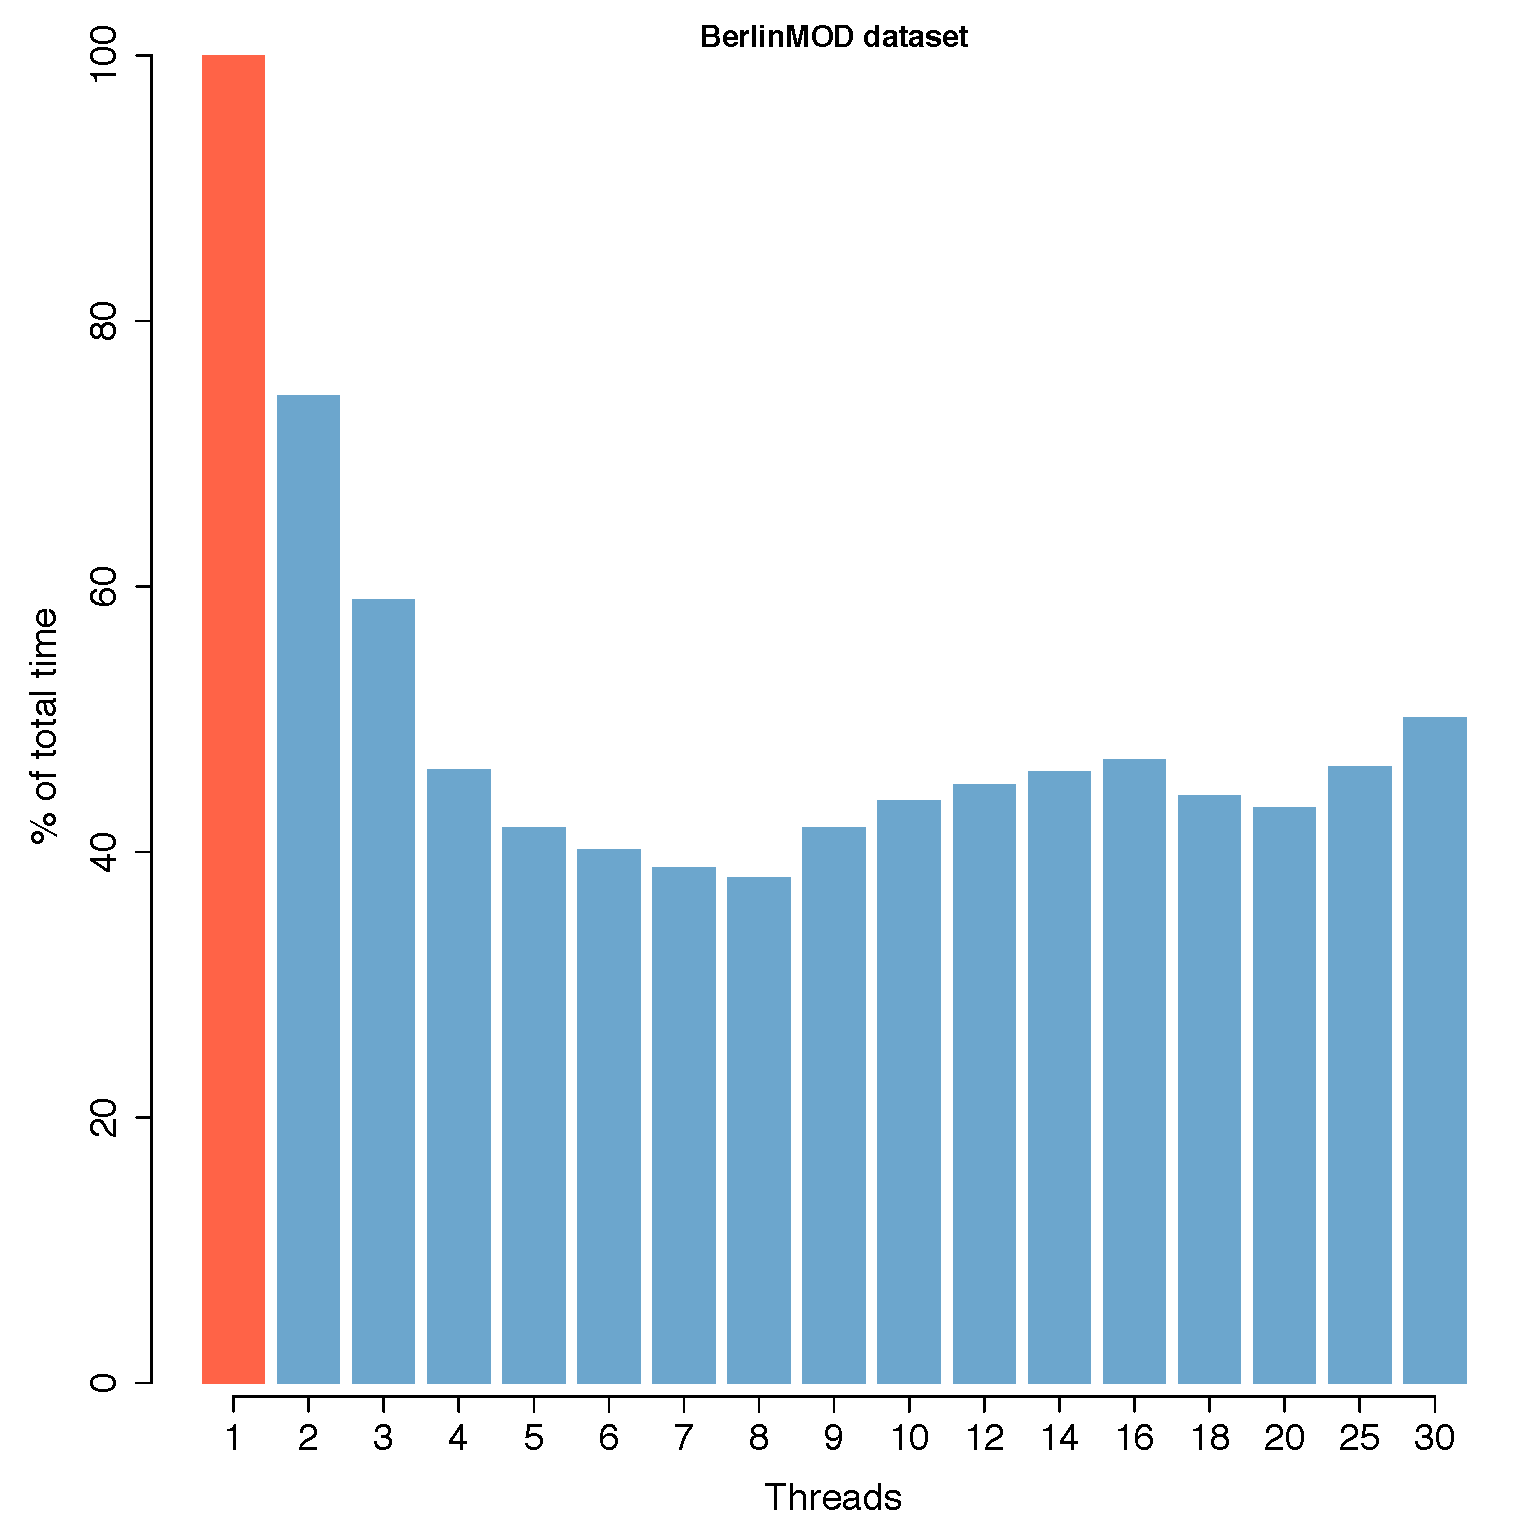
\includegraphics[width=0.7\textwidth]{images/BerlinMOD_thread.eps}
    \caption{Execution time reduction by number of threads for the BerlinMOD dataset}
    \label{fig:berlinmod_threads}
\end{figure}

TDrive is also a large dataset, but not as large as BerlinMOD and its executing time was not as long as the latter.
Based on the results presented in \secref{sec:tdrive}, we chose the parameter that led to the longest executing time
(around 600 seconds): $\mu=4$, $\delta=4$ and $\epsilon=100$. \figref{fig:tdrive_threads} shows tht the results obey the
same pattern that we have been seeing in the previous results: great improvements in the beginning, but stabilizing as
we exceed the number of processing units in the machine. We can also see some slight improvements even when we evaluate
with more than 5 worker threads. We can see in \figref{fig:tdrive_threads} that we were able to reduce the running time
as much as 70\%, when compared to the single threaded model, which is a huge improvement added to those already achieved
in \secref{sec:tdrive}

When it comes to comparing the running time of BitDF MT against BitDF and BFE, we can see that BitDF MT was able to
improve the running time even more than we have seen in \secref{sec:tdrive}. When varying the parameter $\mu$ we could
reduce the execution time by 60\%, as one can see in \figref{fig:tdrive_complete_vary_n}.
\figref{fig:tdrive_complete_vary_g} also shows improvements of 60\%, when compared to BitDF, when varying the parameter
$\epsilon$. The best result though is when we varied the parameter $\delta$, in which we could improve the BitDF running
time by 70\% when executing BitDF MT with both 5 and 7 worker threads, as depicted in
\figref{fig:tdrive_complete_vary_g}.

\begin{figure}[h!]
    \centering
    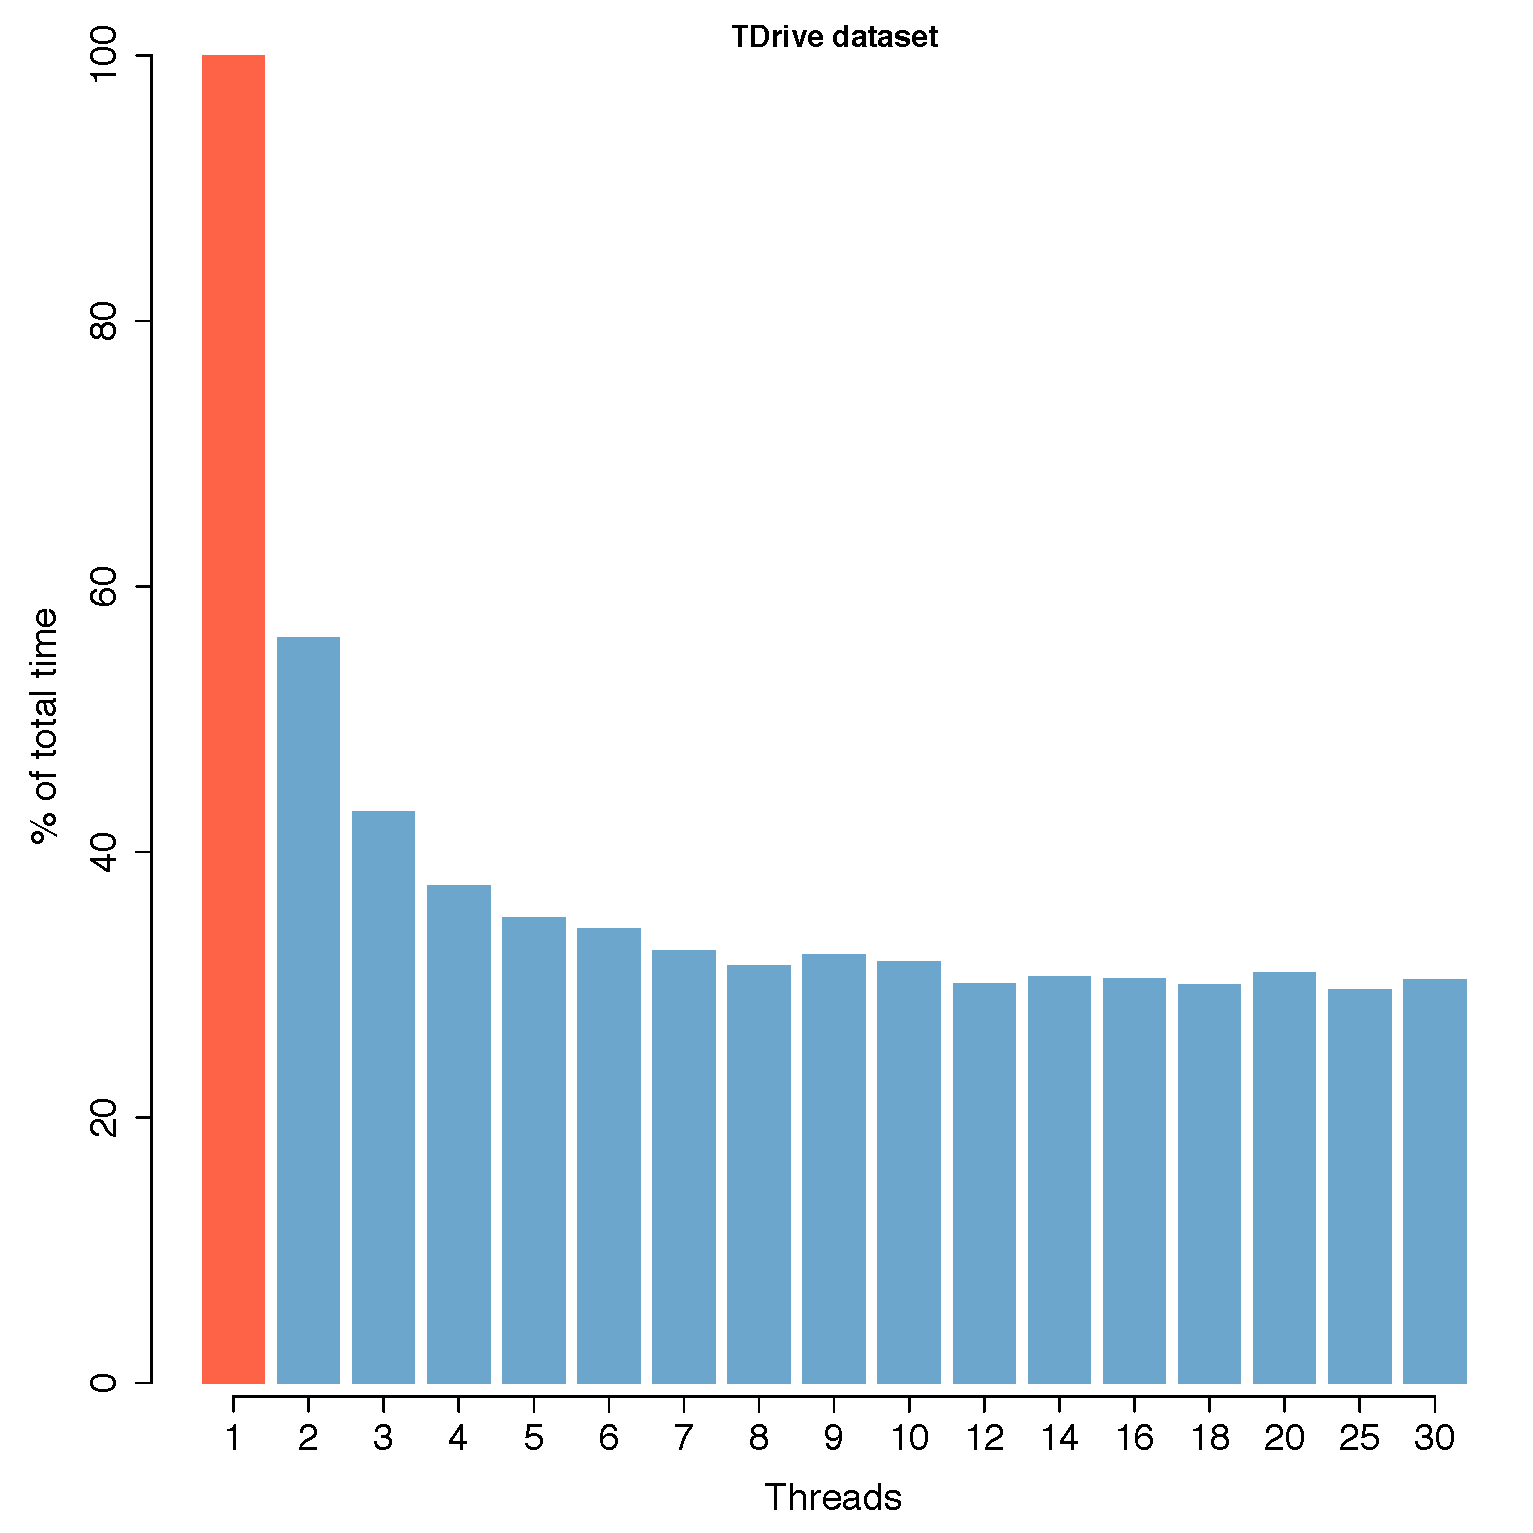
\includegraphics[width=0.7\textwidth]{images/TDrive_thread.eps}
    \caption{Execution time reduction by number of threads for the TDrive dataset}
    \label{fig:tdrive_threads}
\end{figure}

\begin{figure*}[h!]
    \centering
    \begin{subfigure}[t]{0.49\textwidth}
        \includegraphics[width=\textwidth]{images/TDrive_complete_varying_l.eps}
        \caption{$\mu = 4$, $\epsilon = 100$ and $\delta$ varying}
        \label{fig:tdrive_complete_vary_l}
    \end{subfigure}
    \begin{subfigure}[t]{0.49\textwidth}
        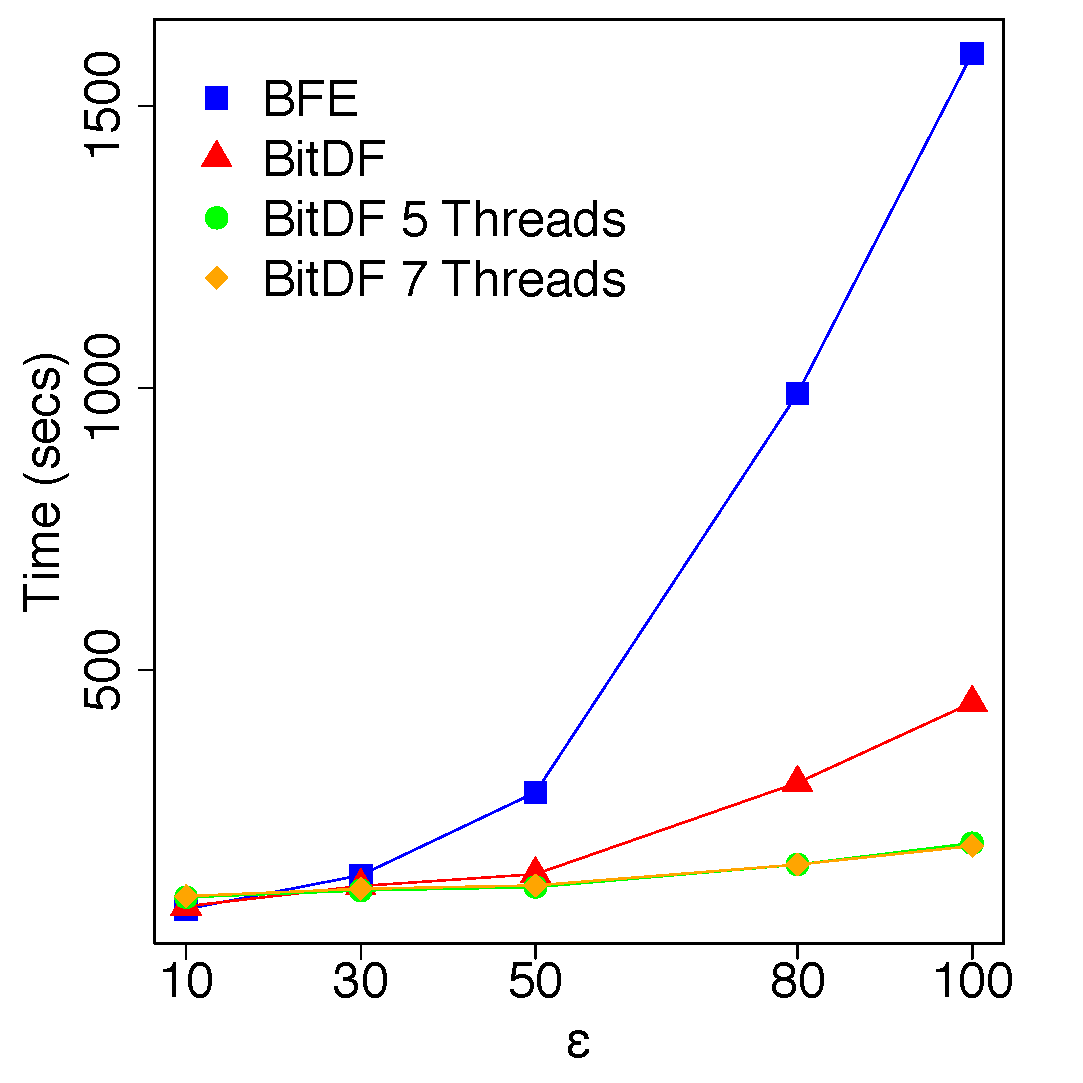
\includegraphics[width=\textwidth]{images/TDrive_complete_varying_g.eps}
        \caption{$\mu = 4$, $\delta = 8$ and $\epsilon$ varying}
        \label{fig:tdrive_complete_vary_g}
    \end{subfigure}
    \caption{Results varying $\delta$ and $\epsilon$ for TDrive dataset}
    \label{fig:tdrive_complete_results}
\end{figure*}

\begin{figure}[h!]
    \centering
    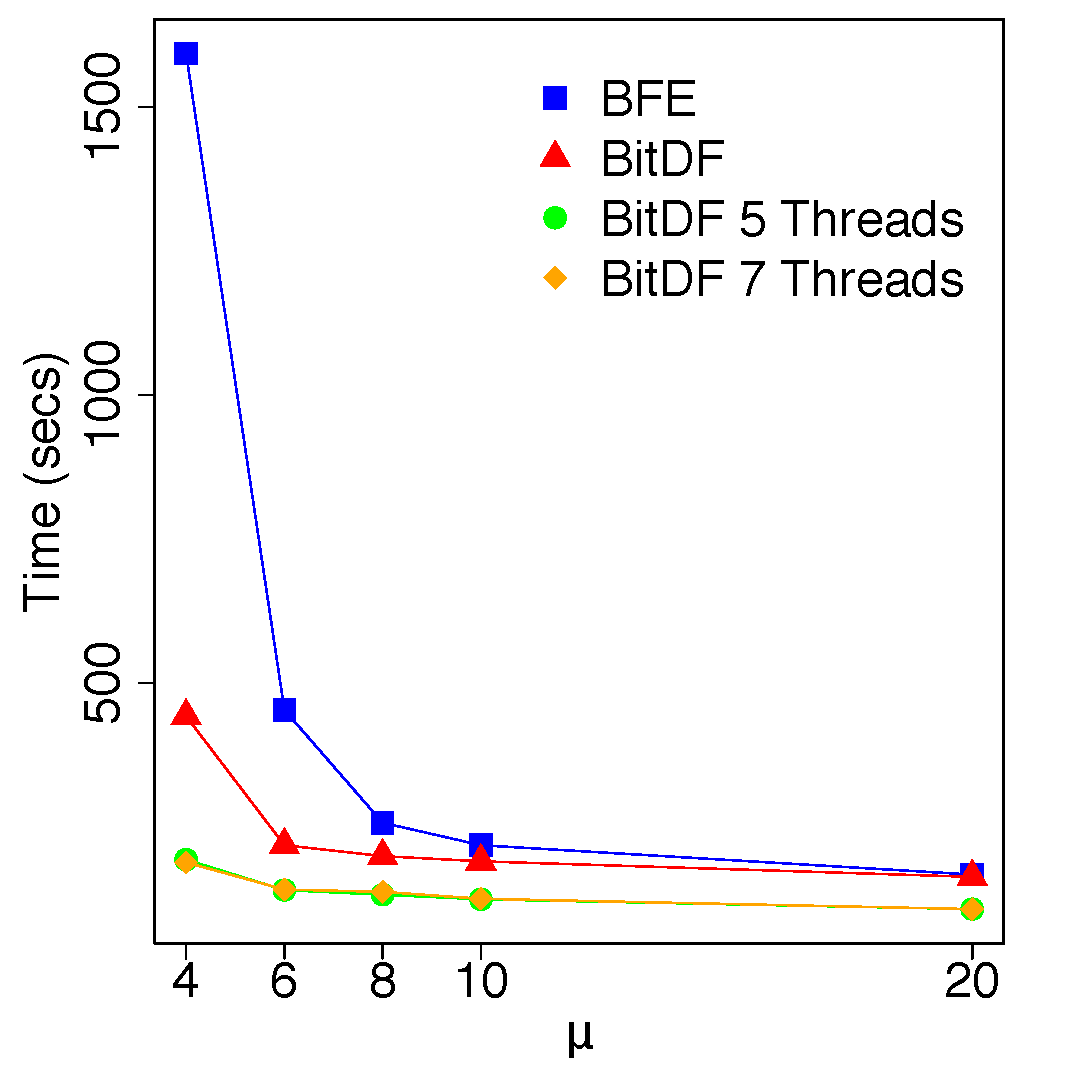
\includegraphics[width=0.5\textwidth]{images/TDrive_complete_varying_n.eps}
    \caption{Results having $\delta = 8$, $\epsilon = 100$ and $\mu$ varying for the TDrive dataset}
    \label{fig:tdrive_complete_vary_n}
\end{figure}

Our last dataset to evaluate is the Brinkhoff synthetic dataset. We were already able to achieve huge running time
improvements with BitDF, but we could achieve even more with BitDF MT. Based on the dataset results
(\secref{sec:brinkhoff}), we chose the running parameters as follows: $\mu=4$, $\delta=4$ and $\epsilon=1200$.
\figref{fig:brinkhoff_threads} shows that we were always able to reduce the BitDF running time even with the number of
worker threads being way higher than the number of available processing units in the machine. That is a result that is
completely different from those that we saw with the previous datasets. Compared with the BitDF run, we could reduce the
running time by 96\%, being that highest cutback achieved with 30 worker threads (60 in total). Given that different
behavior from the other datasets, we took a closer look on it when running with a high number of threads, in order to
try to find out the reason that BitDF MT runs better as the number of worker threads grow. As one can see in
\figref{fig:brinkhoff_disks_threads}, the number of disks that are being generated by the disk threads ($d_i$) are very
close to the final number of disks that are being inserted in the global disk set. That means that the each disk thread
is able to eliminate a lot of repeated and superset disks before returning them to be merged in the global set. Another
thing that is important to note is that the number of disks being generated is really small as time advances, meaning
that the points are more scattered over time, causing less disks to be generated and then less synchronization between
shared queues for each executing thread. Because of that, threads could spend less time blocked waiting for shared data
to become available.

\begin{figure}[h!]
    \centering
    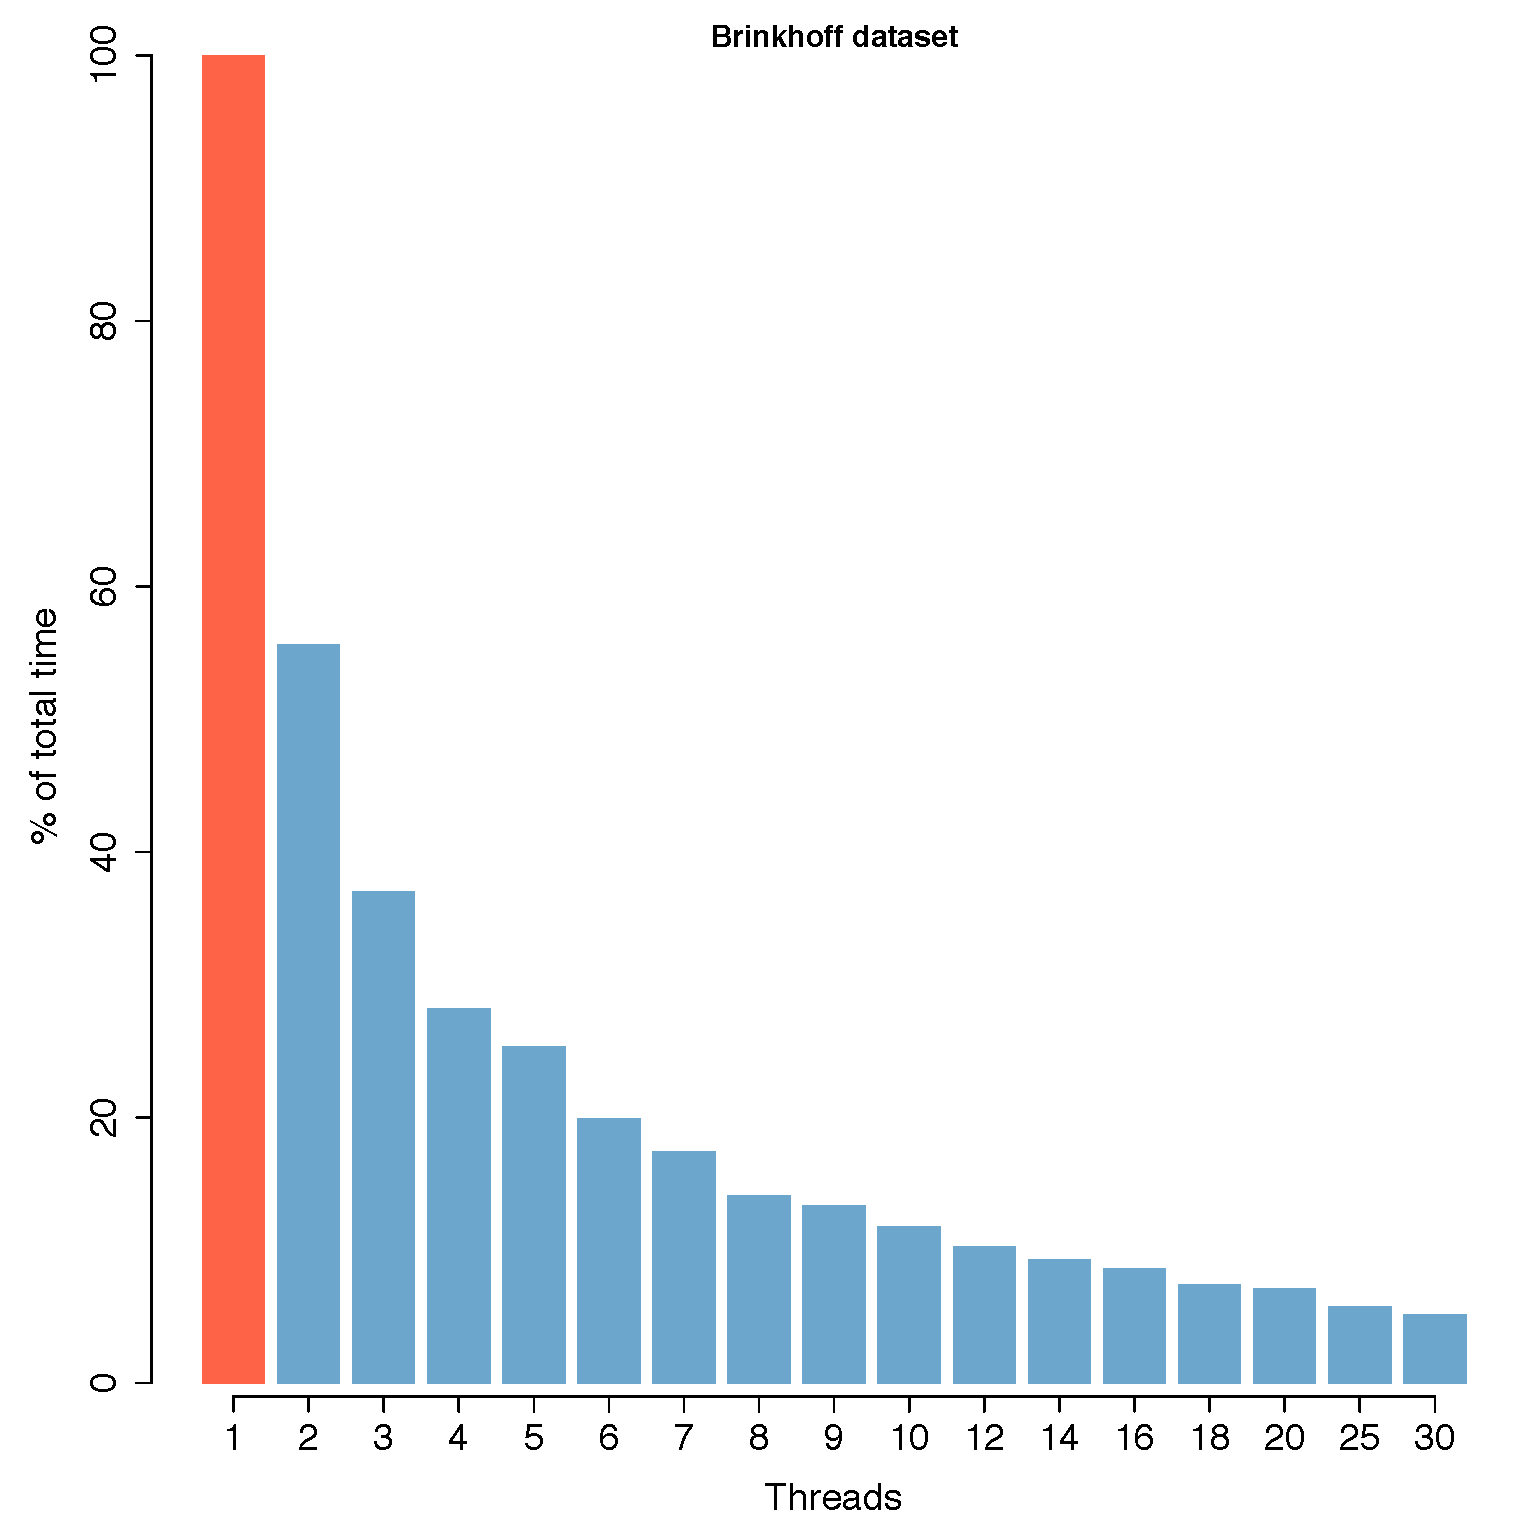
\includegraphics[width=0.7\textwidth]{images/Brinkhoff_thread.eps}
    \caption{Execution time reduction by number of threads for the Brinkhof dataset}
    \label{fig:brinkhoff_threads}
\end{figure}

\begin{figure}[h!]
    \centering
    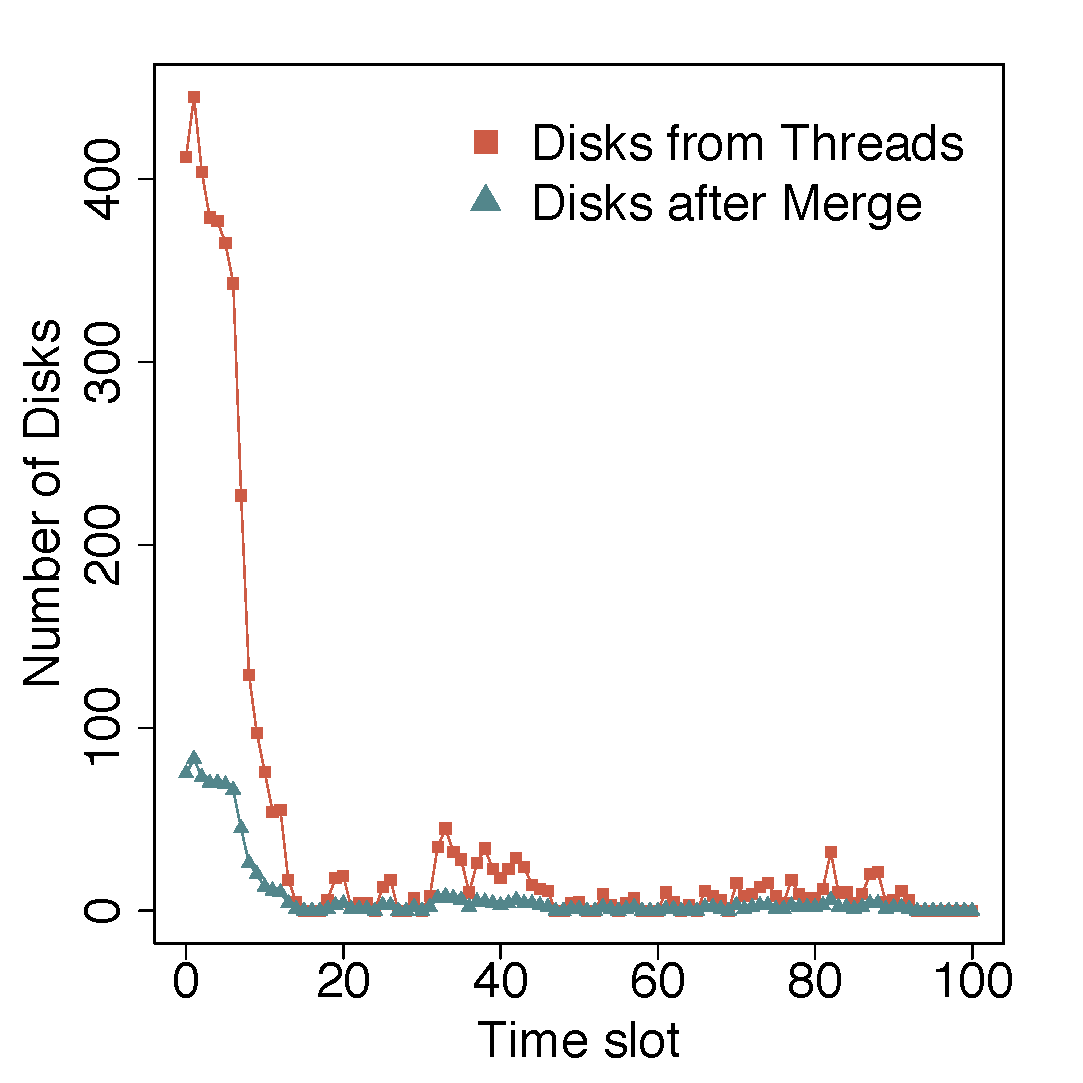
\includegraphics[width=0.5\textwidth]{images/Brinkhoff_disks_threads.eps}
    \caption{Sum of disks generated by the disk threads (red) and number of disks that were inserted in the global disk
        set after subset/superset check (blue), by time slot}
    \label{fig:brinkhoff_disks_threads}
\end{figure}

Despite the reduction in running time of more than 90\% that BitDF was able to achieve, seen in \secref{sec:brinkhoff},
we could reduce that number even more with BitDF MT. It is difficult to see the actual difference between the running
time of BitDF and BitDF MT, due to the slowness of BFE in that dataset, which is causing the y axis range to be very
wide. However, BitDF MT with 5 and 7 worker threads could reduce the time of BitDF by 82\% when varying the $\mu$
parameters, as shown in \figref{fig:brinkhoff_complete_vary_n}. When varying the $\epsilon$ parameter, BitDF MT with 5
and 7 worker threads could also decrease the BitDF running time by 82\%. \figref{fig:brinkhoff_complete_vary_g} shows
that when we varying the $\delta$ parameter, good results could be achieve as wel. When running with 5 worker threads,
BitDF MT could outperform BitDF by 76\%, whereas by running with 7 worker threads, BitDF MT could be better by 85\%.

\begin{figure*}[h!]
    \centering
    \begin{subfigure}[t]{0.49\textwidth}
        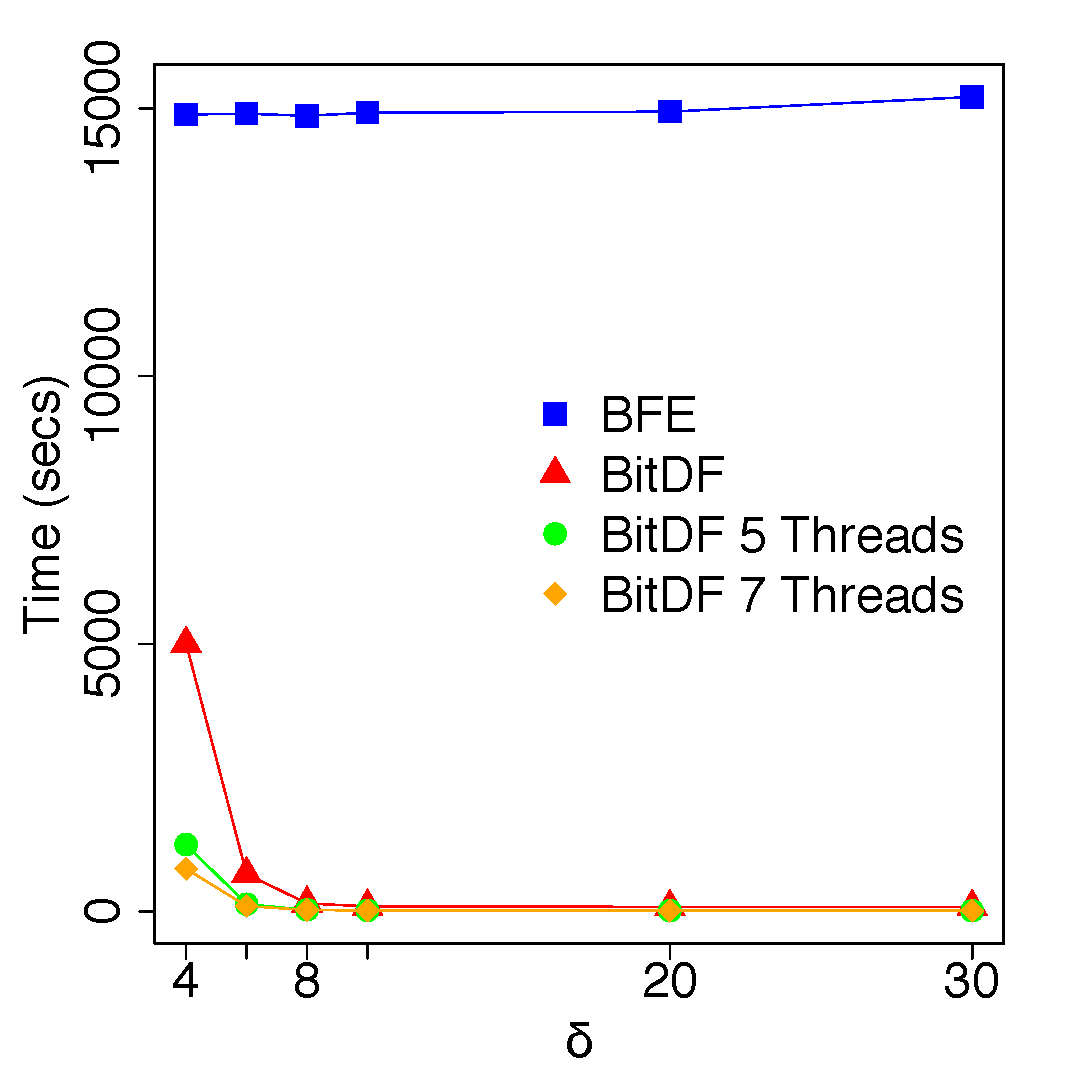
\includegraphics[width=\textwidth]{images/Brinkhoff_complete_varying_l.eps}
        \caption{$\mu = 4$, $\epsilon = 100$ and $\delta$ varying}
        \label{fig:brinkhoff_complete_vary_l}
    \end{subfigure}
    \begin{subfigure}[t]{0.49\textwidth}
        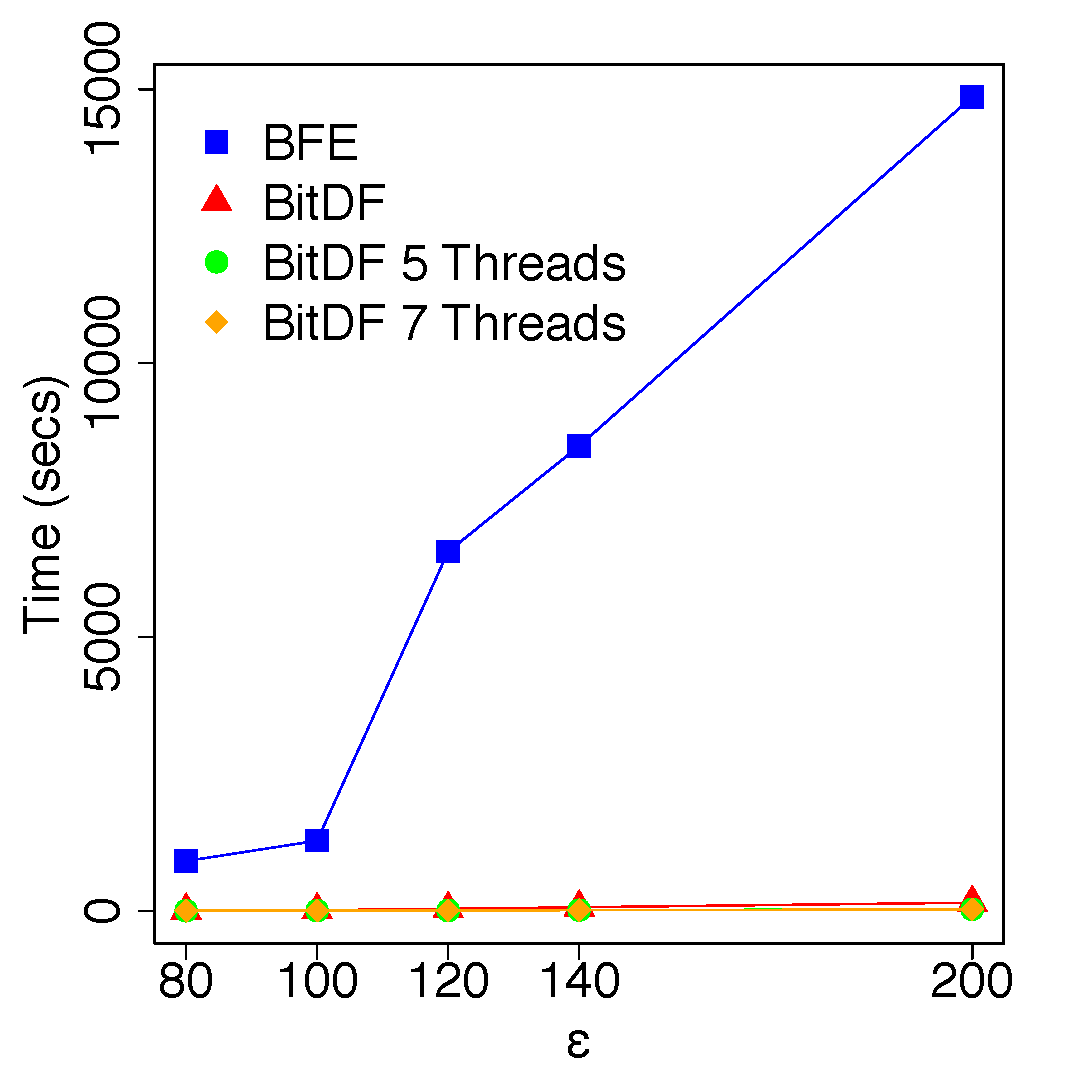
\includegraphics[width=\textwidth]{images/Brinkhoff_complete_varying_g.eps}
        \caption{$\mu = 4$, $\delta = 8$ and $\epsilon$ varying}
        \label{fig:brinkhoff_complete_vary_g}
    \end{subfigure}
    \caption{Results varying $\delta$ and $\epsilon$ for Brinkhoff dataset}
    \label{fig:brinkhoff_complete_results}
\end{figure*}

\begin{figure}[h!]
    \centering
    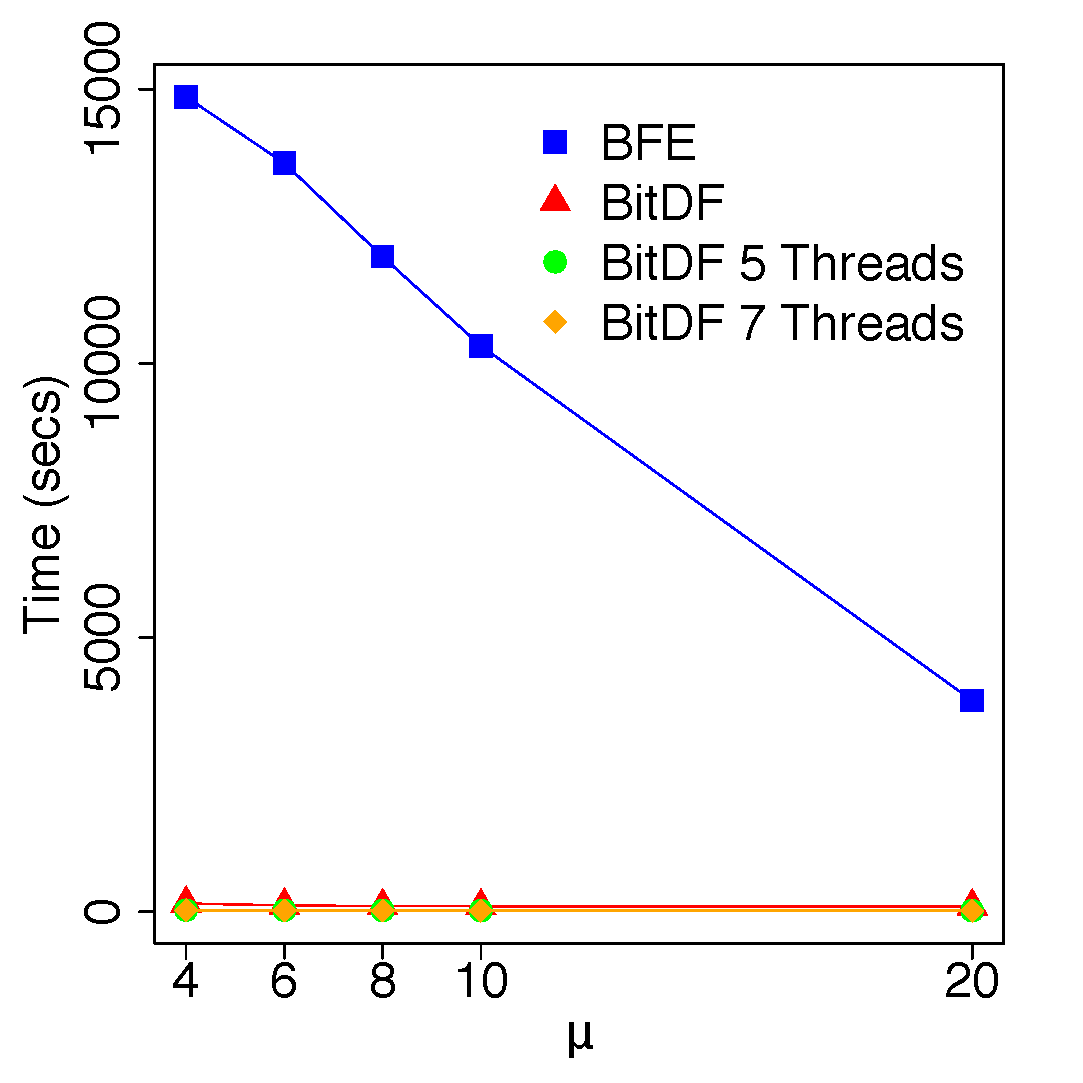
\includegraphics[width=0.5\textwidth]{images/Brinkhoff_complete_varying_n.eps}
    \caption{Results having $\delta = 8$, $\epsilon = 100$ and $\mu$ varying for the Brinkhoff dataset}
    \label{fig:brinkhoff_complete_vary_n}
\end{figure}

In this section we could show that a somewhat simple remodeling in a system's architecture could lead to tremendous
running time improvements, by taking advantage of the multi-core paradigm. Our results show that we could reduce the
running time by as much as 96\%, when choosing the correct number of worker threads and the correct separation of work
that can be parallelized.
